\documentclass[../structure.tex]{subfiles}
\begin{document}
\chapter{Results}
\hspace{2em}After implementing non-rigid ICP, we test the code we have developed to assess the algorithm. The device used for this test is \textit{HP EliteBook 820 G3}, as shown in figure \{\ref{fig:OS}\} and the operating system used was \textit{Windows 10 Enterprise x64}
\\
\begin{figure}[h!]
\centering

\includegraphics[scale=1.2, frame]{009_os}
\captionsetup{justification=centering}
\caption{The device specification used for testing}
\label{fig:OS}
\end{figure}

The number of samples used for testing is four with eleven pathways (bundles) in each side of the brain. The data is collected by \textbf{\textit{UKB Universitätsklinikum Bonn}}.
% Statistic
\begin{center}
\begin{table}[h!]
	\begin{tabular}{| c | c  c  c | c  c  c |}
	%\begin{tabular}{*7c}
	\toprule
	&\multicolumn{3}{c}{Tracts}&\multicolumn{3}{c}{Points}\\
Pathways&Average&Max&Min&Average&Max&Min\\
\midrule
%\hline
ATR&266.75&603&106&26443.875&69283&9623\\
rostrum&1853.375&2020&1633&162936.625&188143&137536\\
Cing&1103.375&1369&872&167488.25&244088&100762\\
CST&1649.25&2044&1476&235265.375&308769&170535\\
Fornix&399&497&308&26618&37142&16703\\
genu&2134.5&2333&1967&166567.625&236384&144492\\
IFOF&862.875&985&774&128850.875&162086&90424\\
ILF&3751&4392&2950&566332.25&673060&367155\\
SLF&1333.125&1633&1044&174943.5&251994&105245\\
splenium&2209.625&2335&2063&206526.875&244341&182993\\
VTA&327.625&679&150&27784.125&54904&14982\\
\bottomrule
	\end{tabular}
\caption{The statistics of tracts (streamlines) and points}
\label{table:data}
\end{table}
\end{center}

The test starts by reading the template and target bundles from \textit{ply} files, whereas the template bundle is the Thalamic Radiation (ATR) on the right side and the target bundle is the left side of the ATR from the same patient. Then we visualize two graphs and plot the distances between correspondences points in histograms before and after applying PCA. Depending on the result we have and whether PCA improved the alignment or not, we decide whether to use PCA or not; if PCA improves the alignment, then it is used, otherwise we skip PCA. The figures \{\ref{fig:hist_original}\} \{\ref{fig:img_original}\} \{\ref{fig:hist_PCA}\} \{\ref{fig:img_PCA}\} below show visual orientations and histograms before and after PCA.

\begin{figure}[h!]
\centering
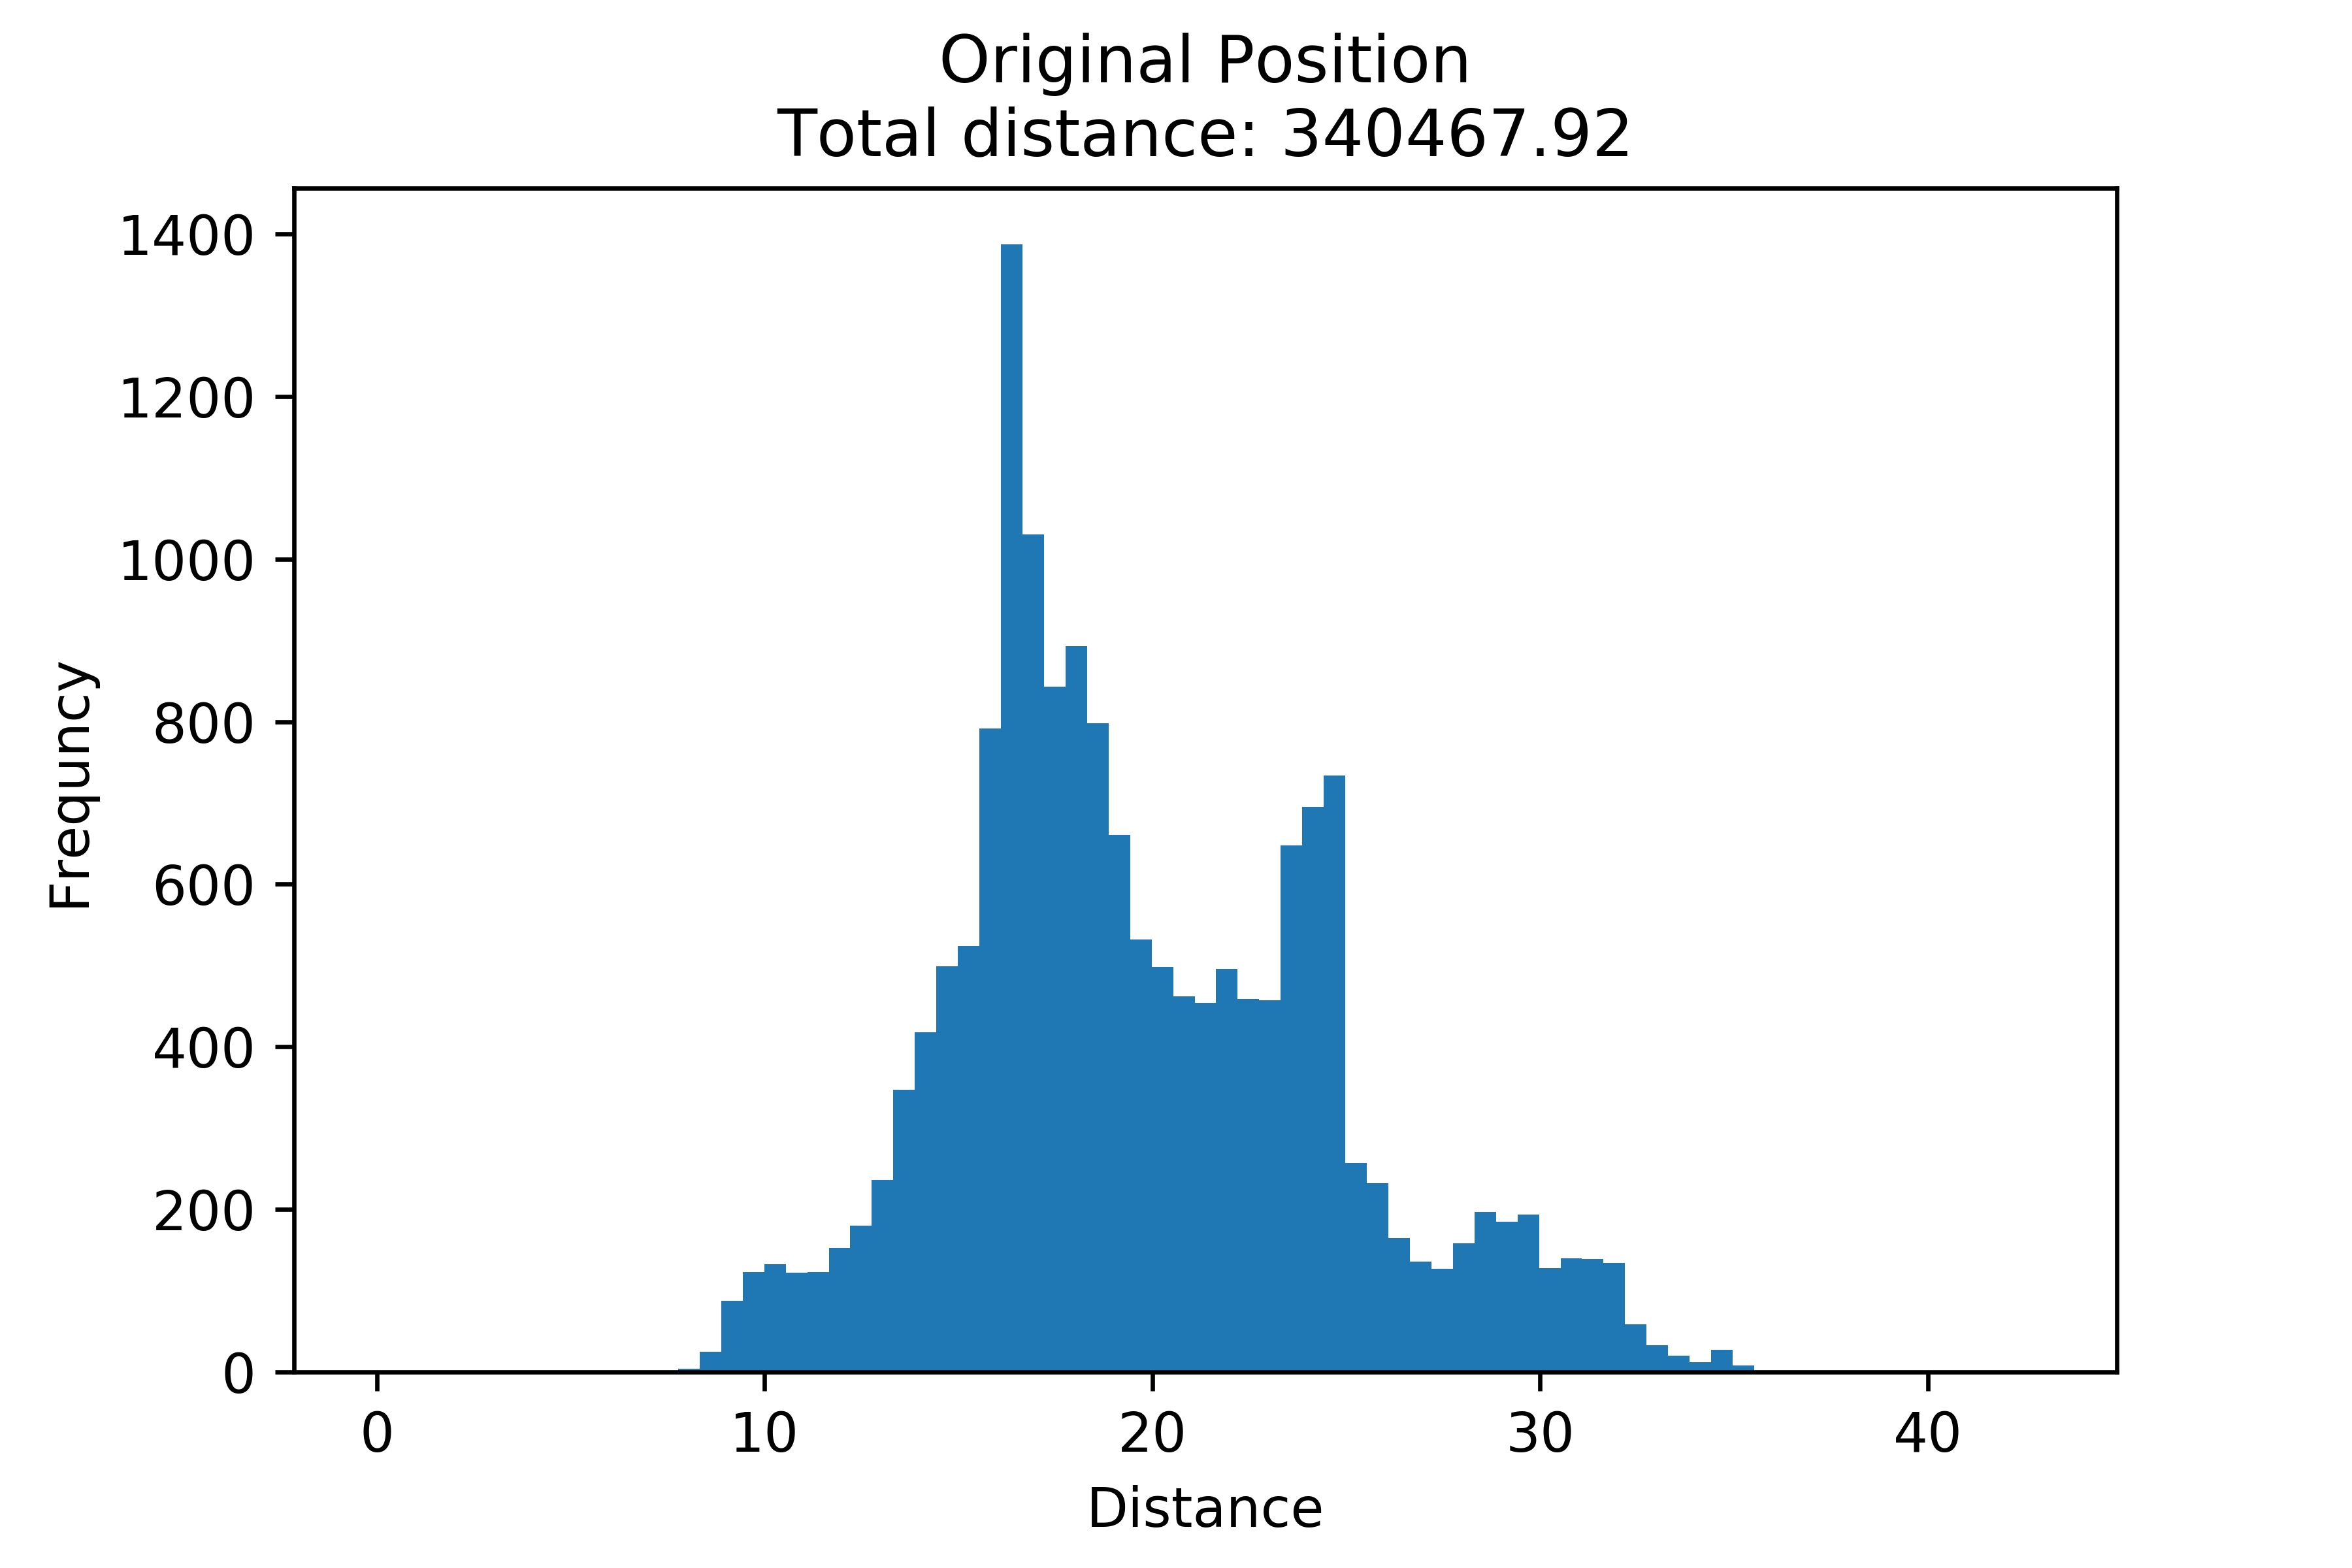
\includegraphics[scale=.9]{101_hist_original}
\captionsetup{justification=centering}
\caption{The original distances histogram}
\label{fig:hist_original}
\end{figure}

\begin{figure}[h!]
\centering
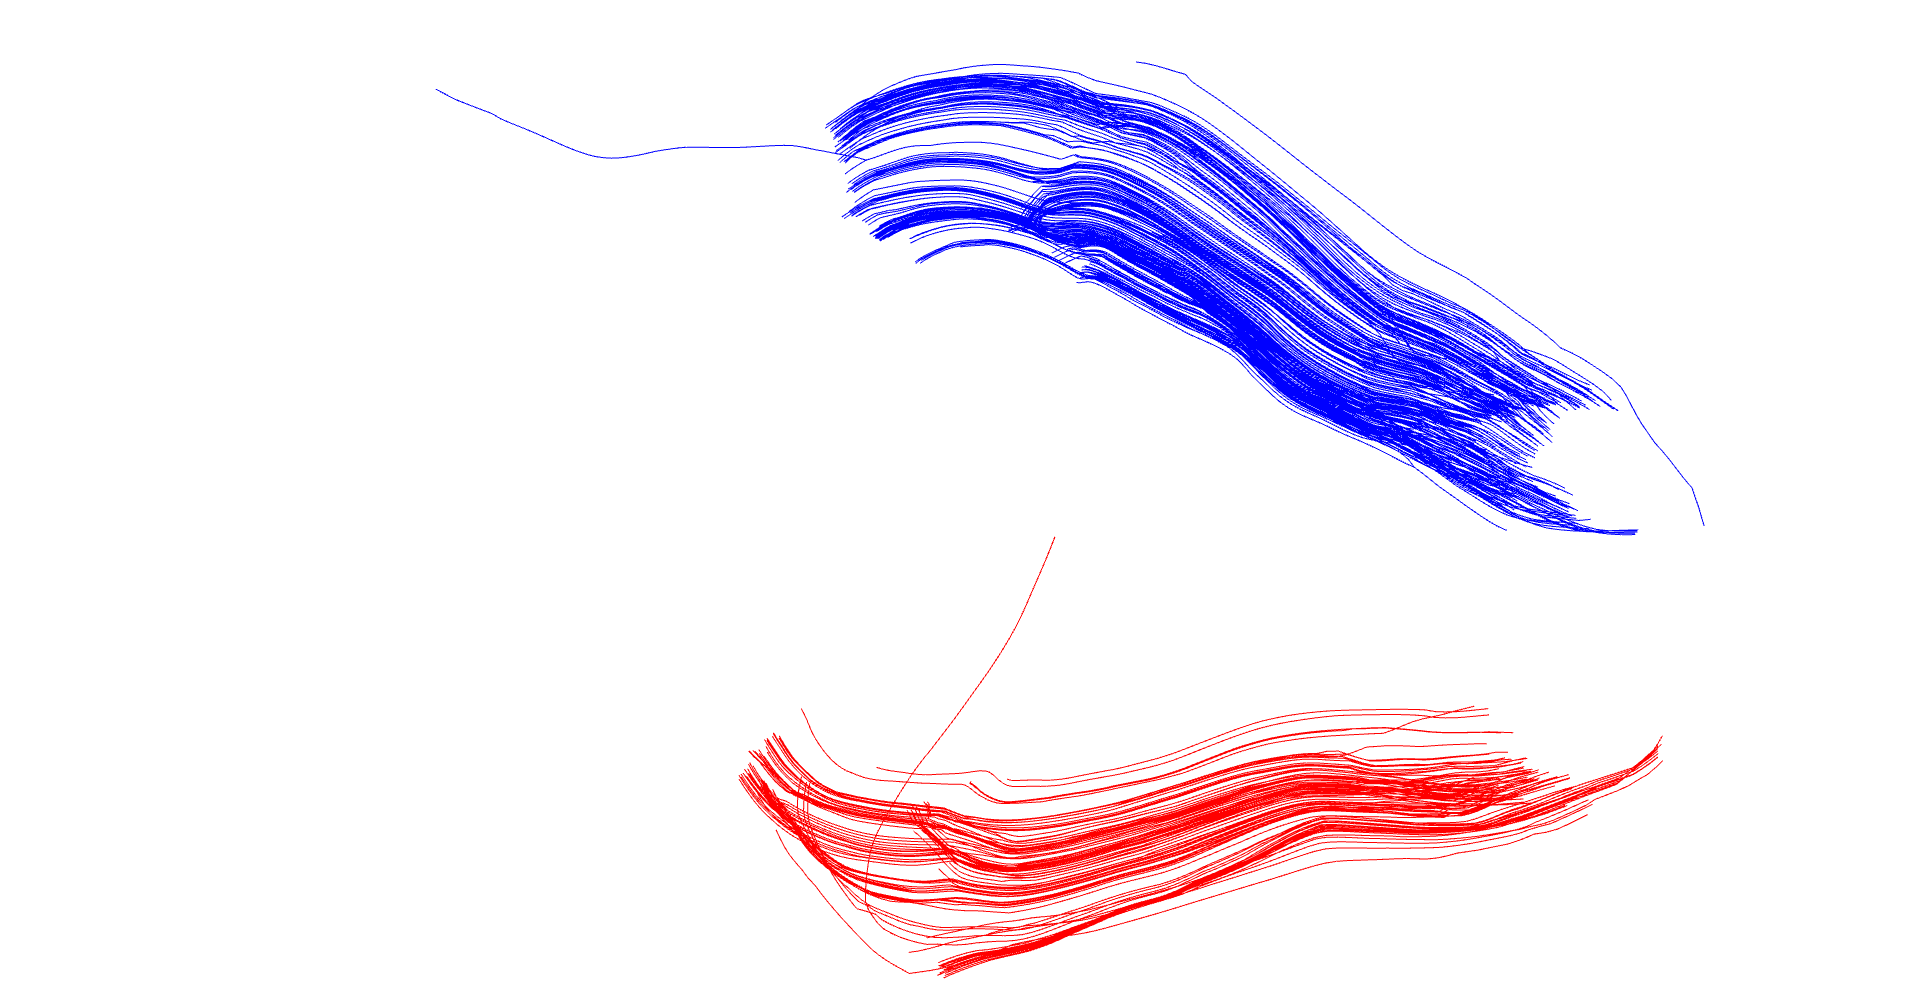
\includegraphics[scale=.7]{101_img_original}
\captionsetup{justification=centering}
\caption{The original orientation}
\label{fig:img_original}
\end{figure}
\pagebreak
\begin{figure}[h!]
\centering
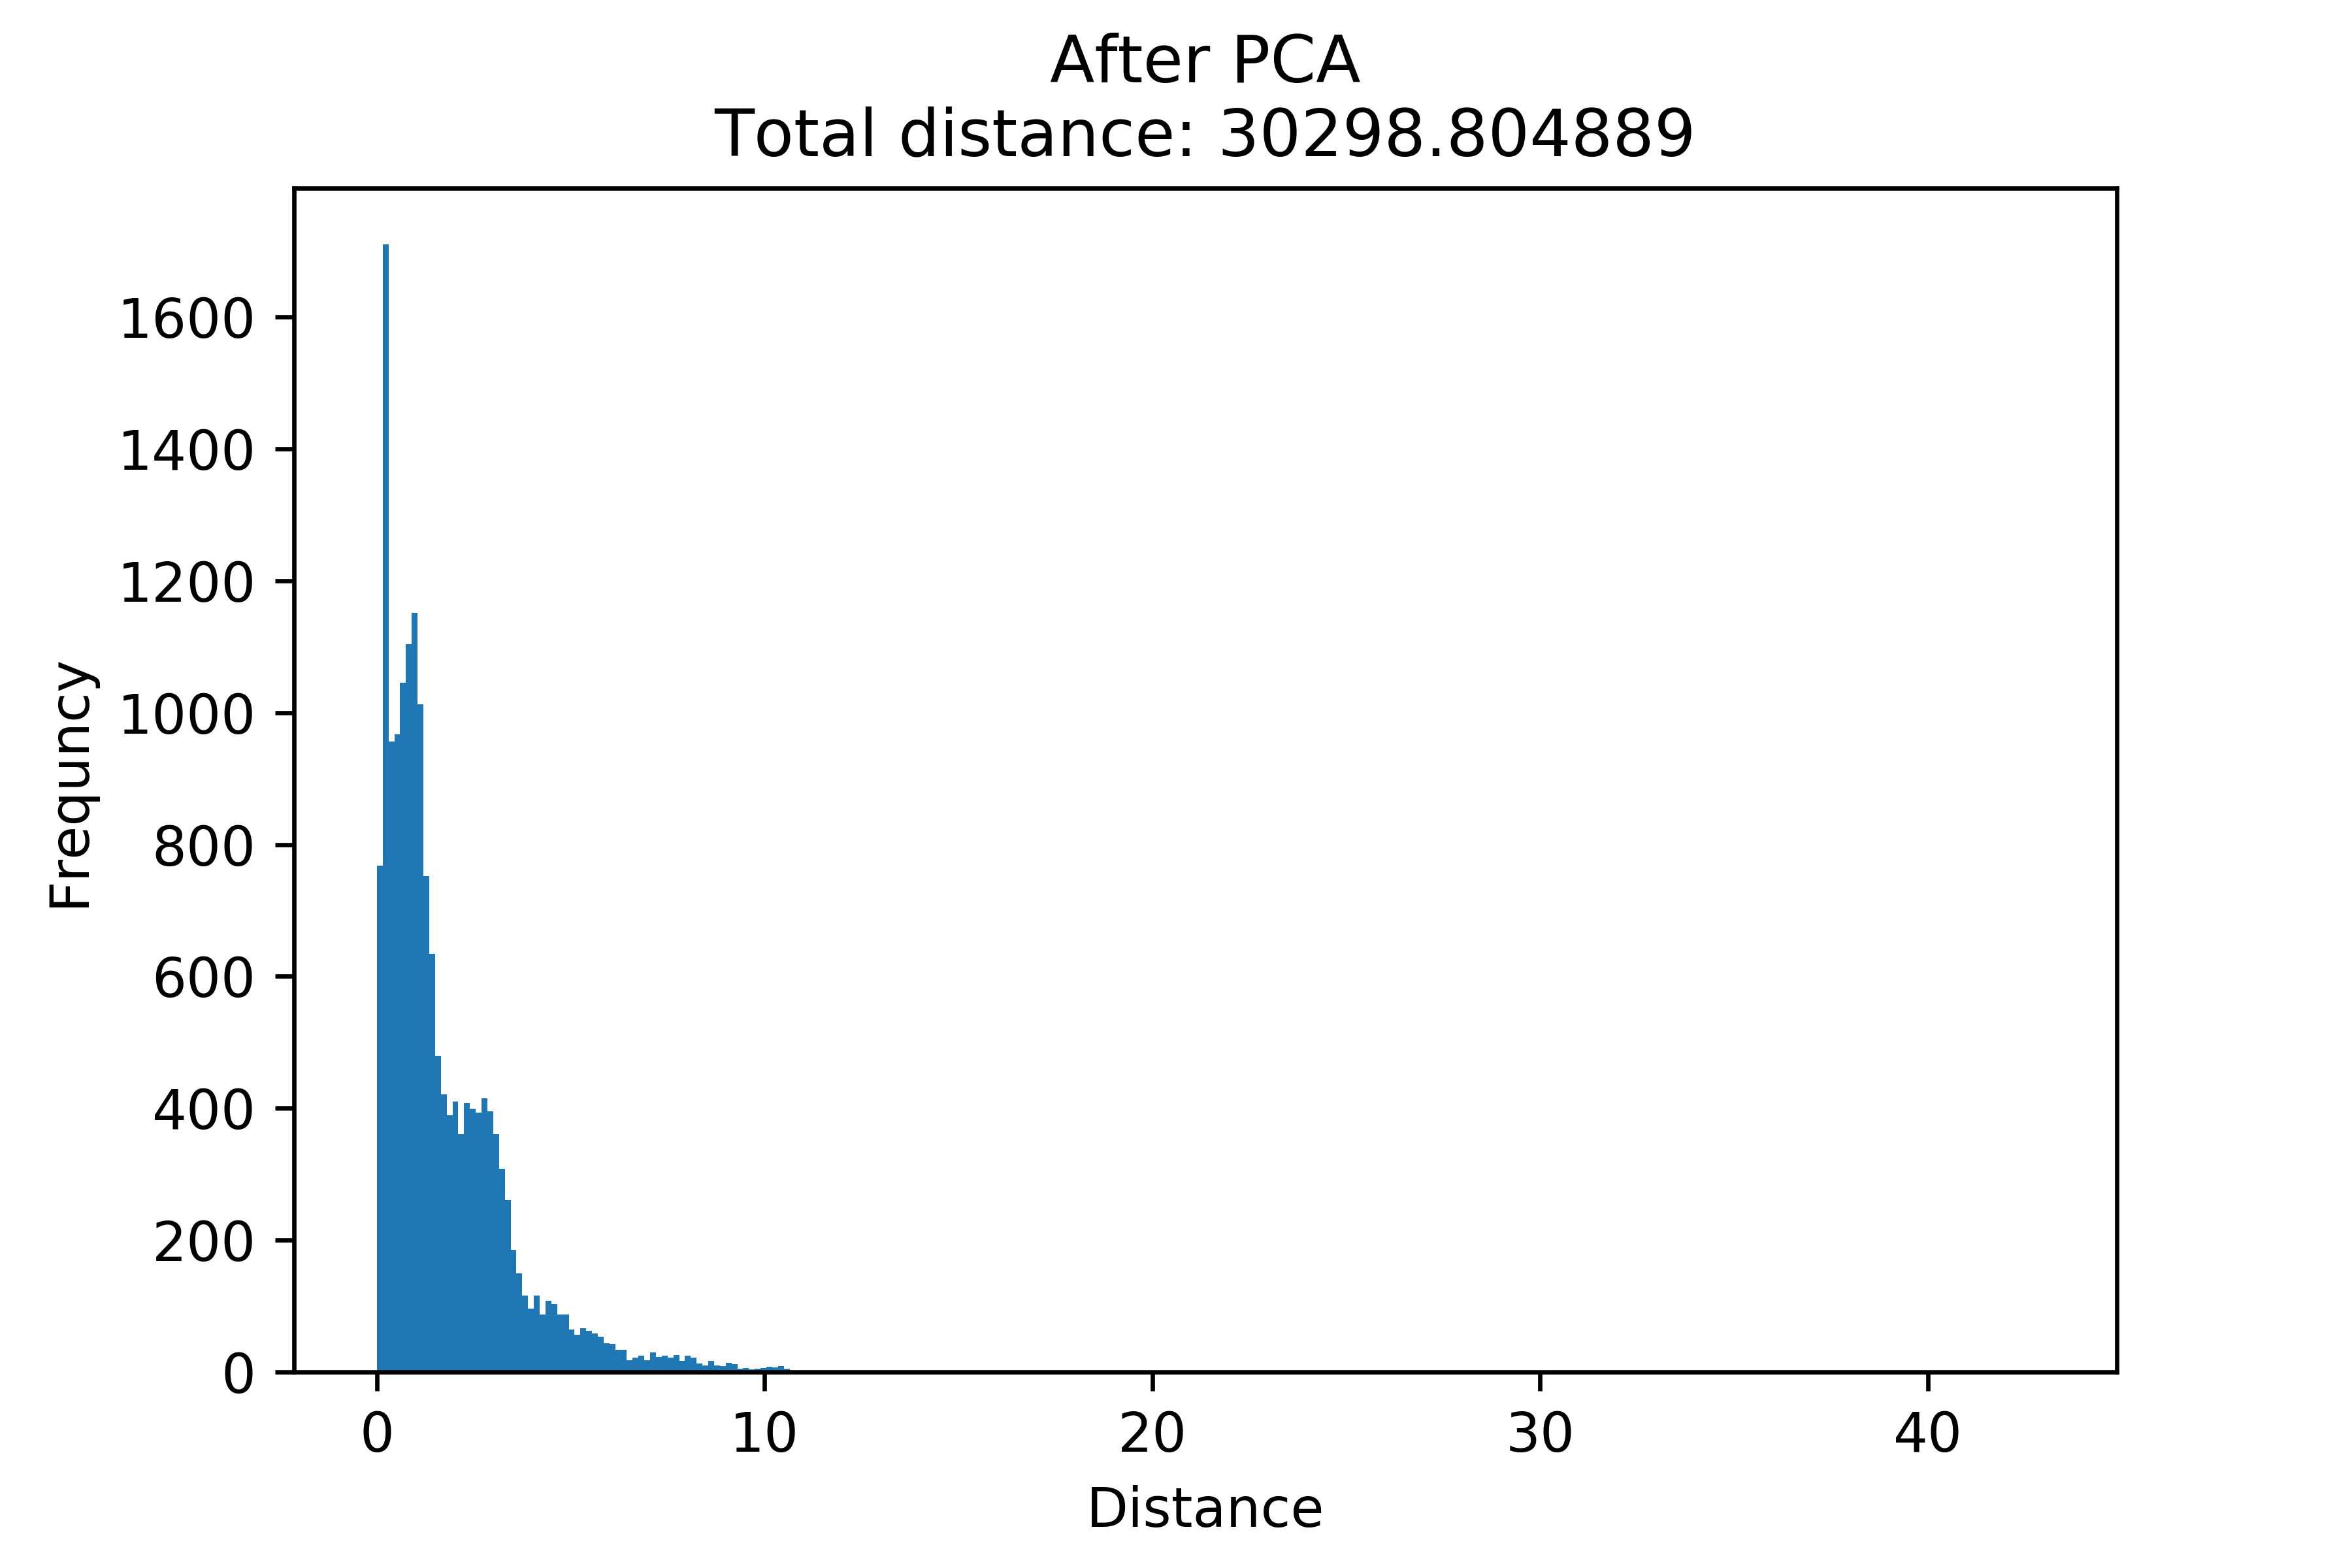
\includegraphics[scale=1]{101_hist_PCA}
\captionsetup{justification=centering}
\caption{The distances histogram after PCA}
\label{fig:hist_PCA}
\end{figure}

\begin{figure}[h!]
\centering
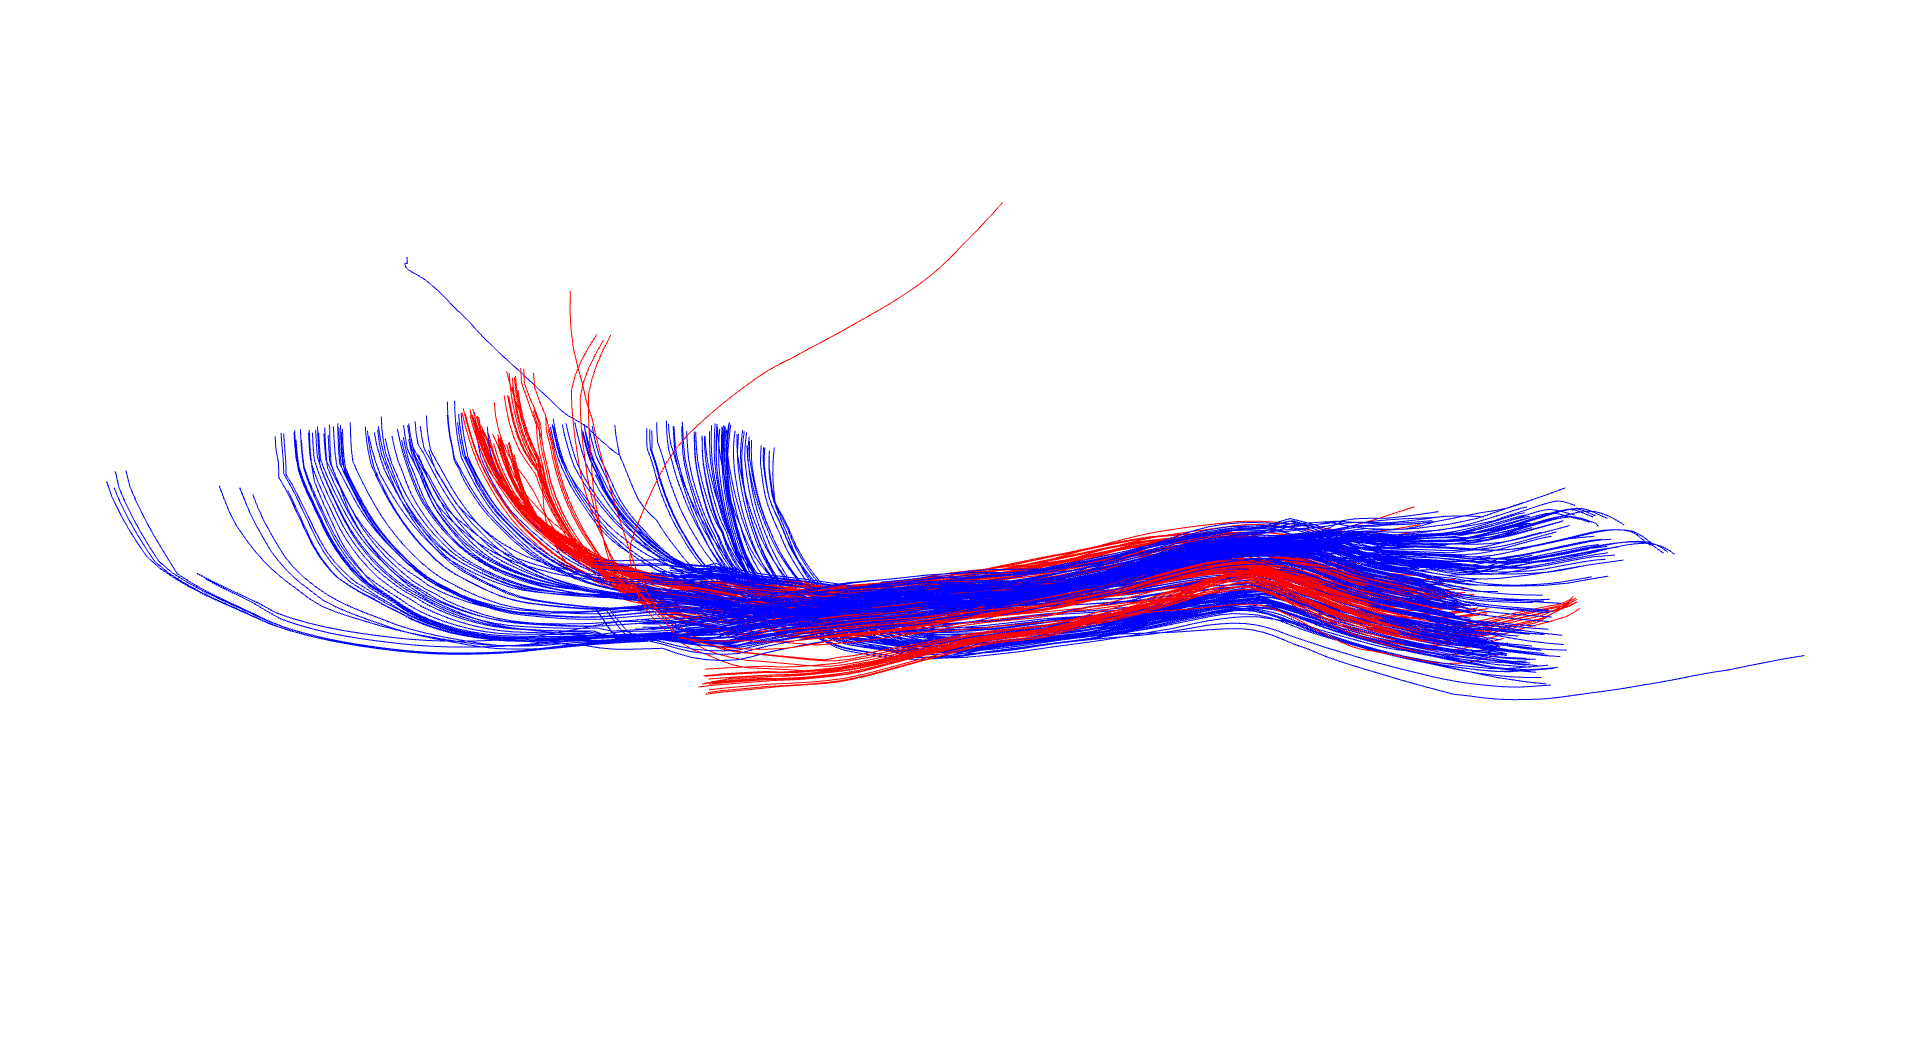
\includegraphics[scale=.3]{101_img_PCA}
\captionsetup{justification=centering}
\caption{The Orientation after PCA}
\label{fig:img_PCA}
\end{figure}
\pagebreak
%\vspace{2em}
When we decide whether to use PCA or not, we select the threshold depending on the histogram. In this case, as we decide to use PCA, we select a threshold equal to seven and around 98\% of points will be included as correspondences. In other words, 98\% of the weight matrix $W$ will be \textit{ones}, as explained in chapter \textit{Methods and implementation}. Then we run \textit{LSQR} to solve the cost function, as illustrated in the previous chapter \textit{Method and Implementation}, and produce the results seen in figures \{\ref{fig:hist_ICP}\} \{\ref{fig:img_ICP}\} below. Later we compare our results with non-linear method called \textit{Dipy} 

\begin{figure}[h!]
\centering
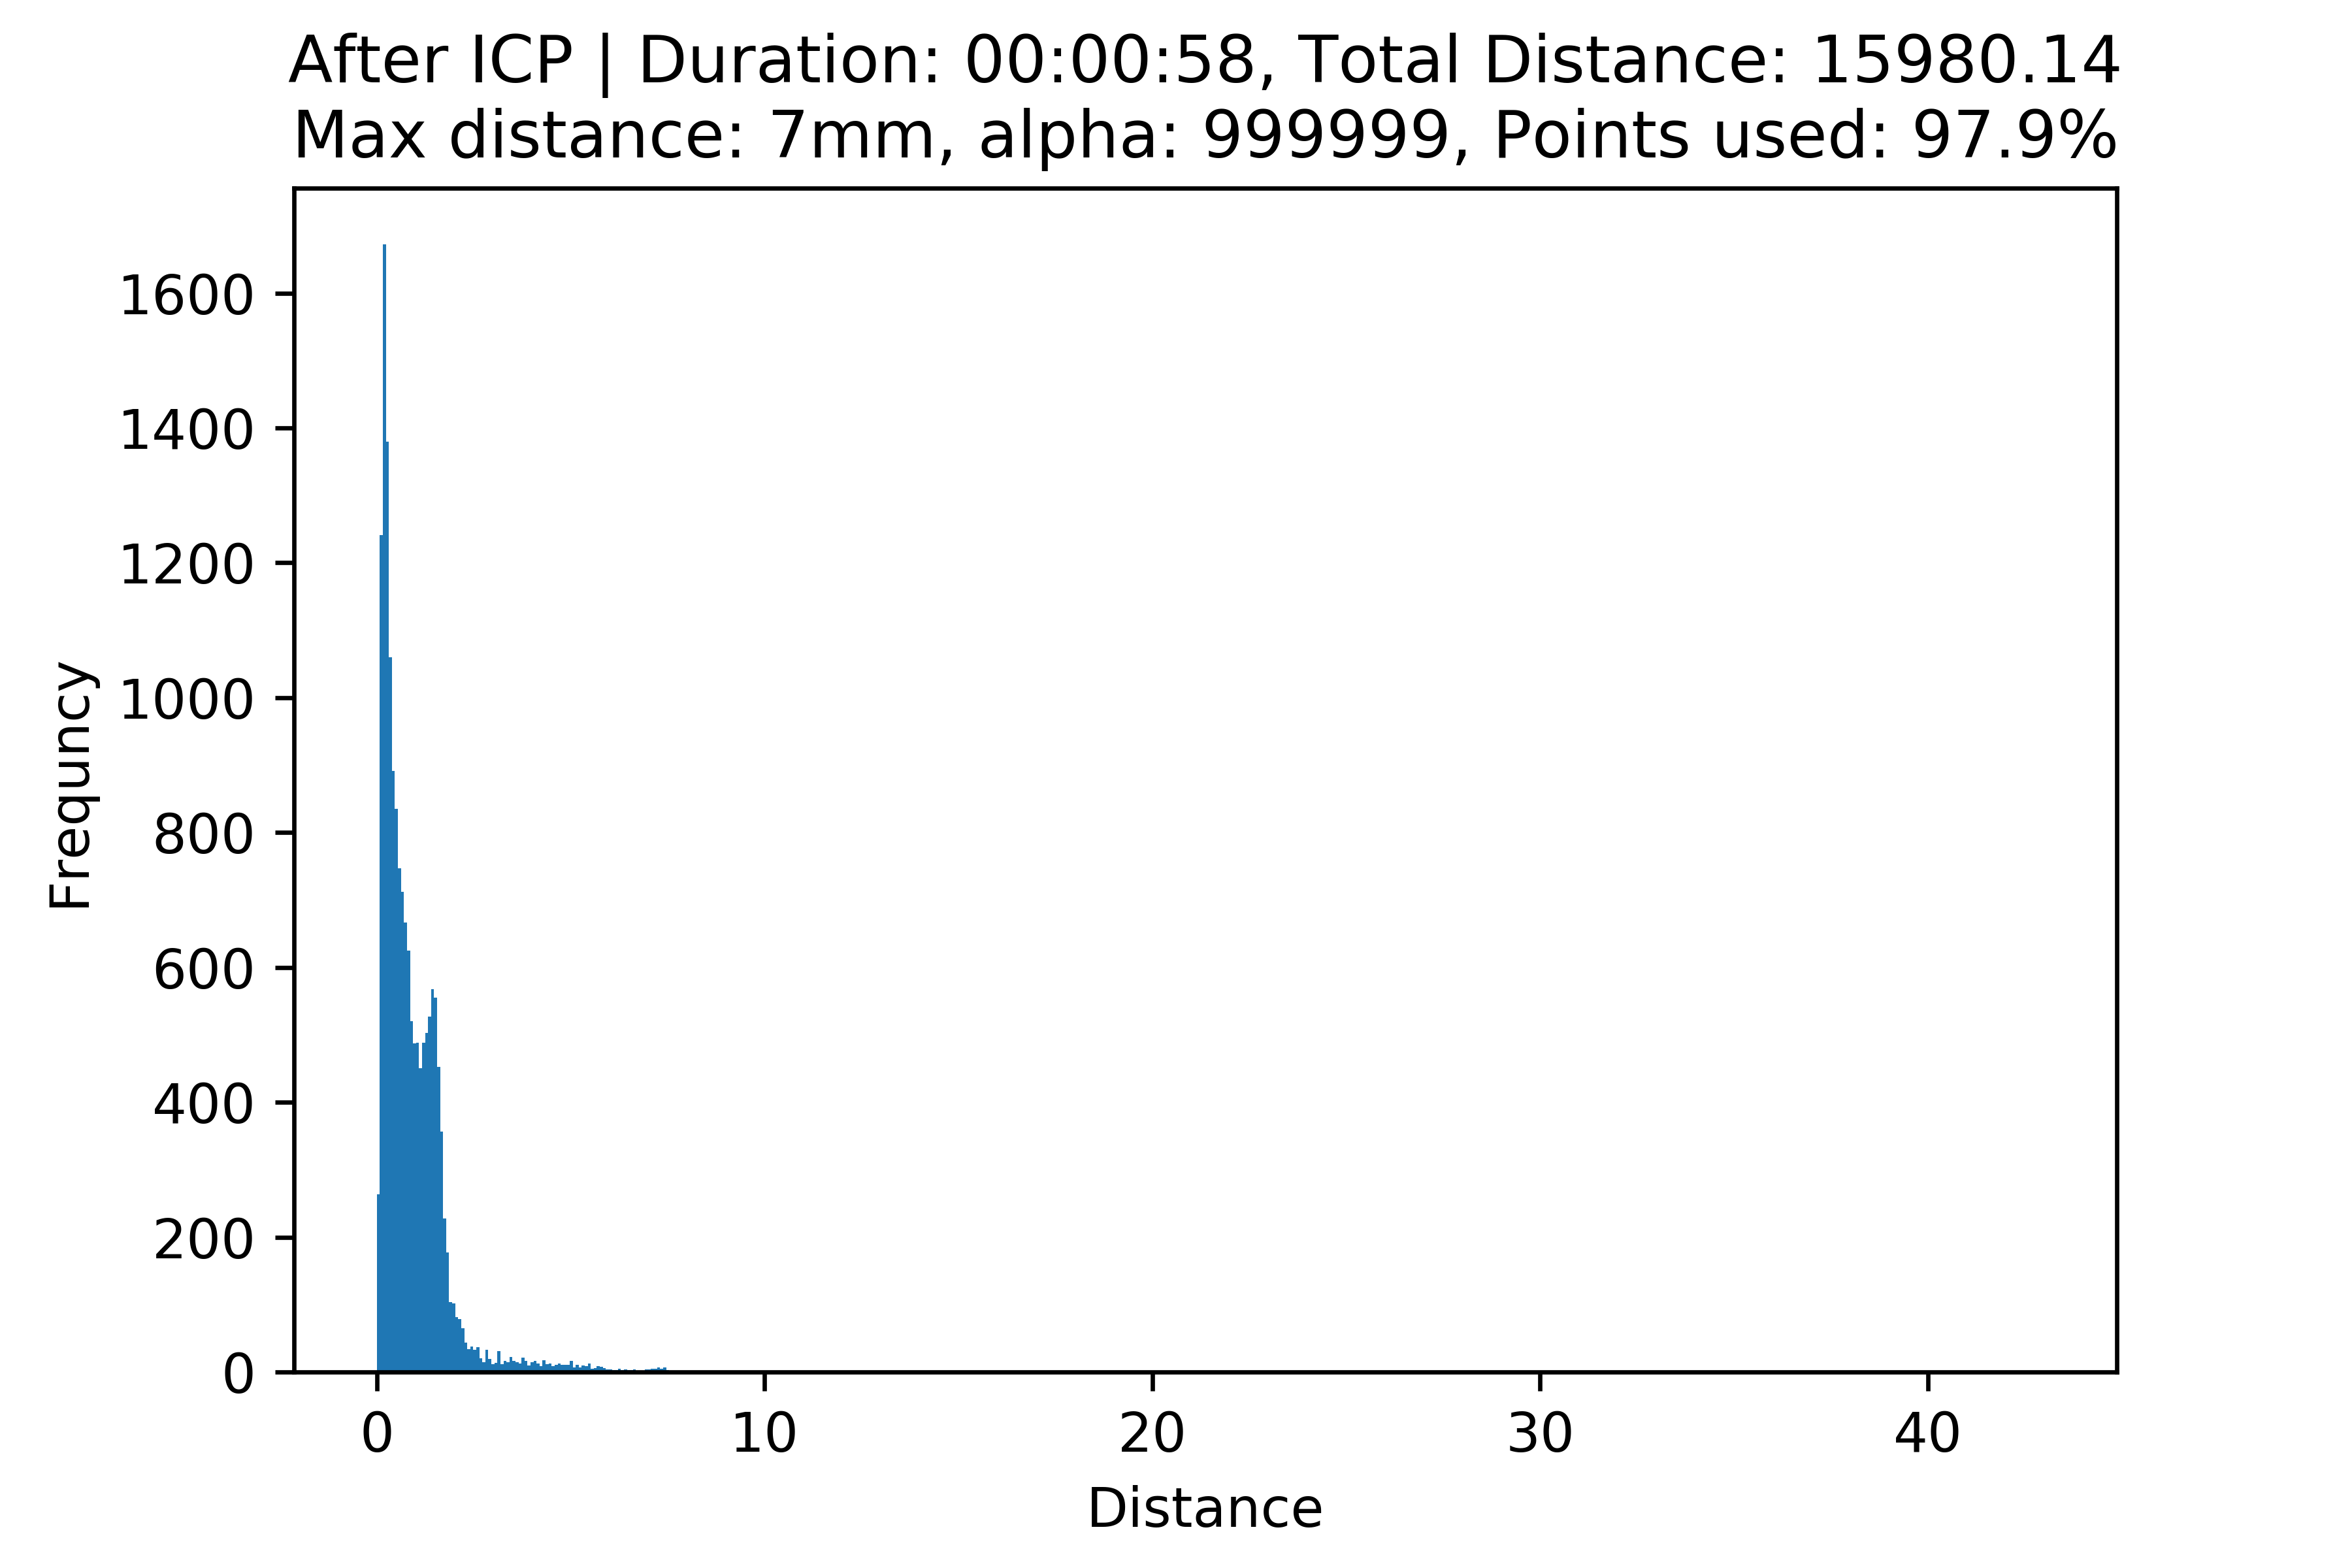
\includegraphics[scale=1]{101_hist_ICP}
\captionsetup{justification=centering}
\caption{The distances histogram after ICP}
\label{fig:hist_ICP}
\end{figure}

\begin{figure}[h!]
\centering
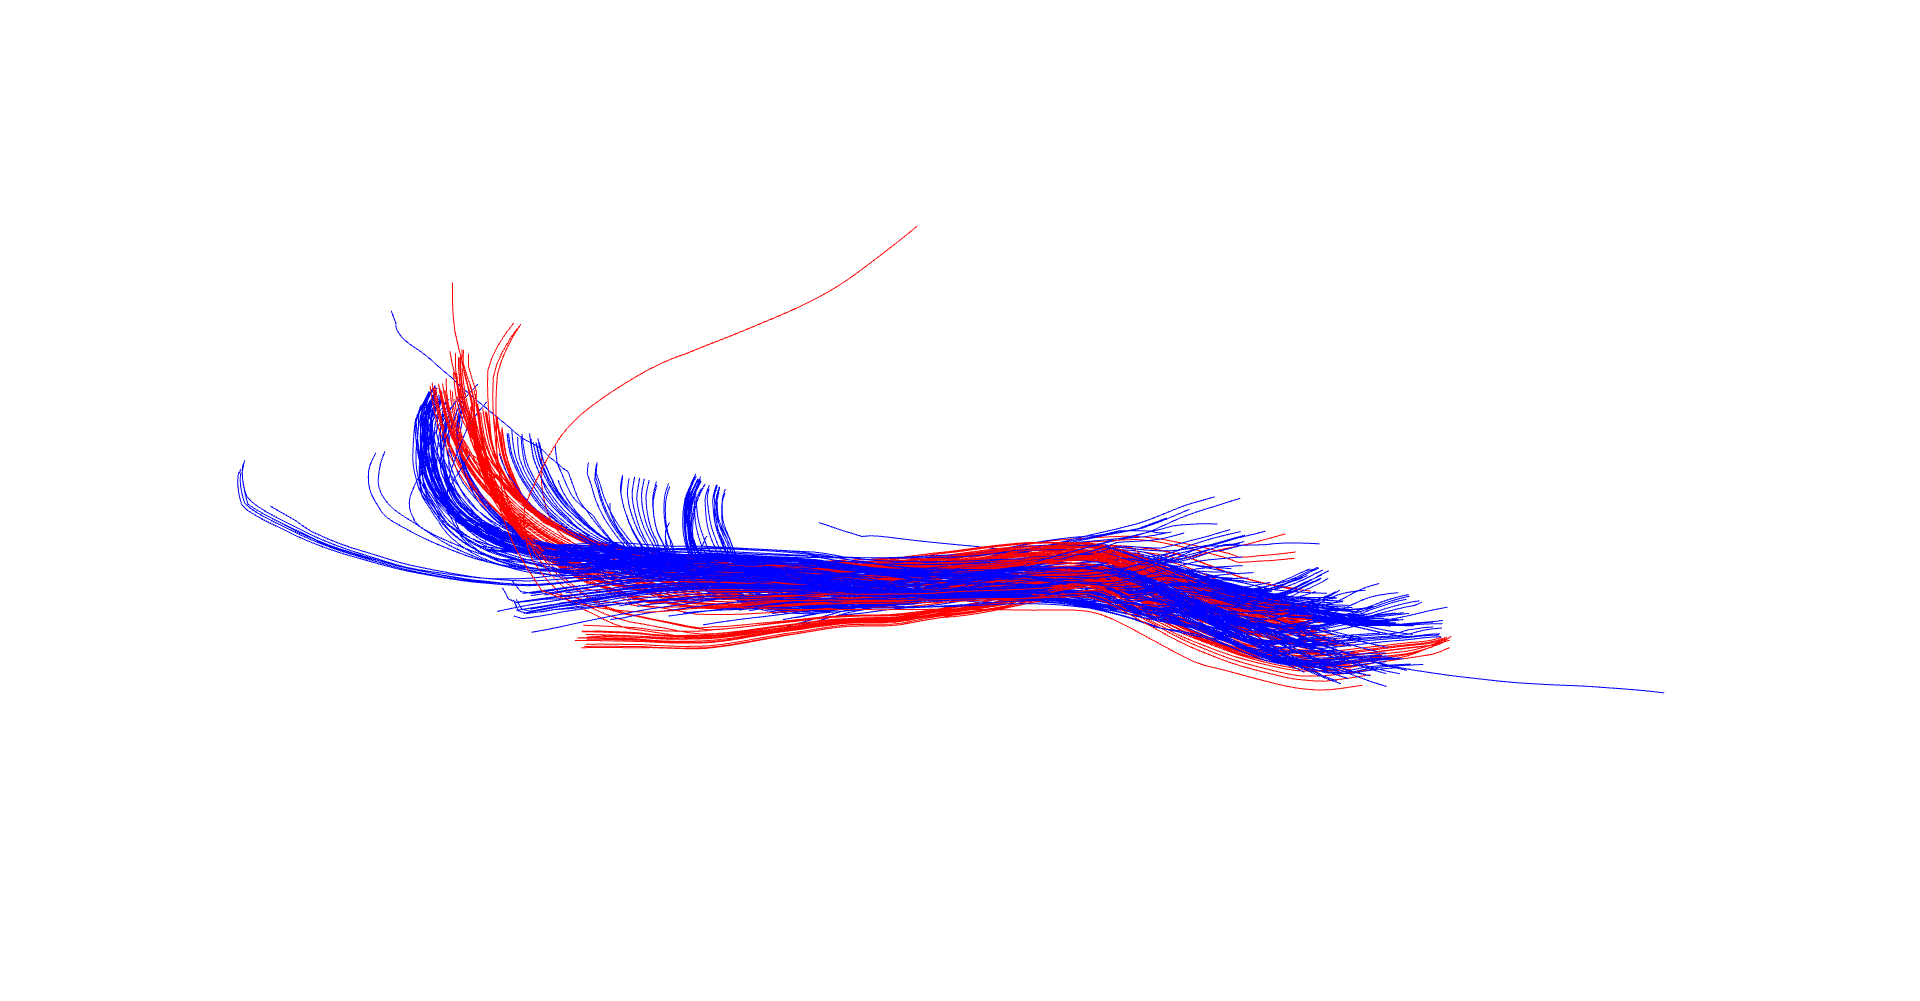
\includegraphics[scale=.4]{101_img_ICP}
\captionsetup{justification=centering}
\caption{The Orientation after ICP}
\label{fig:img_ICP}
\end{figure}
\pagebreak
We align the same bundles with the method discussed in \cite{ODonnell2012} and implemented in \textit{DIPY dipy.align.streamlinear.StreamlineLinearRegistration}. The method gets the initial orientation by bringing both graphs to the origin point of the 3D euclidean space, but it does not take care of the initial alignment. Therefore, we use the PCA tool that we develop to get the initial alignment and produce the results shown in figures \{\ref{fig:dipy_hist}\} \{\ref{fig:img_dipy}\}

\begin{figure}[h!]
\centering
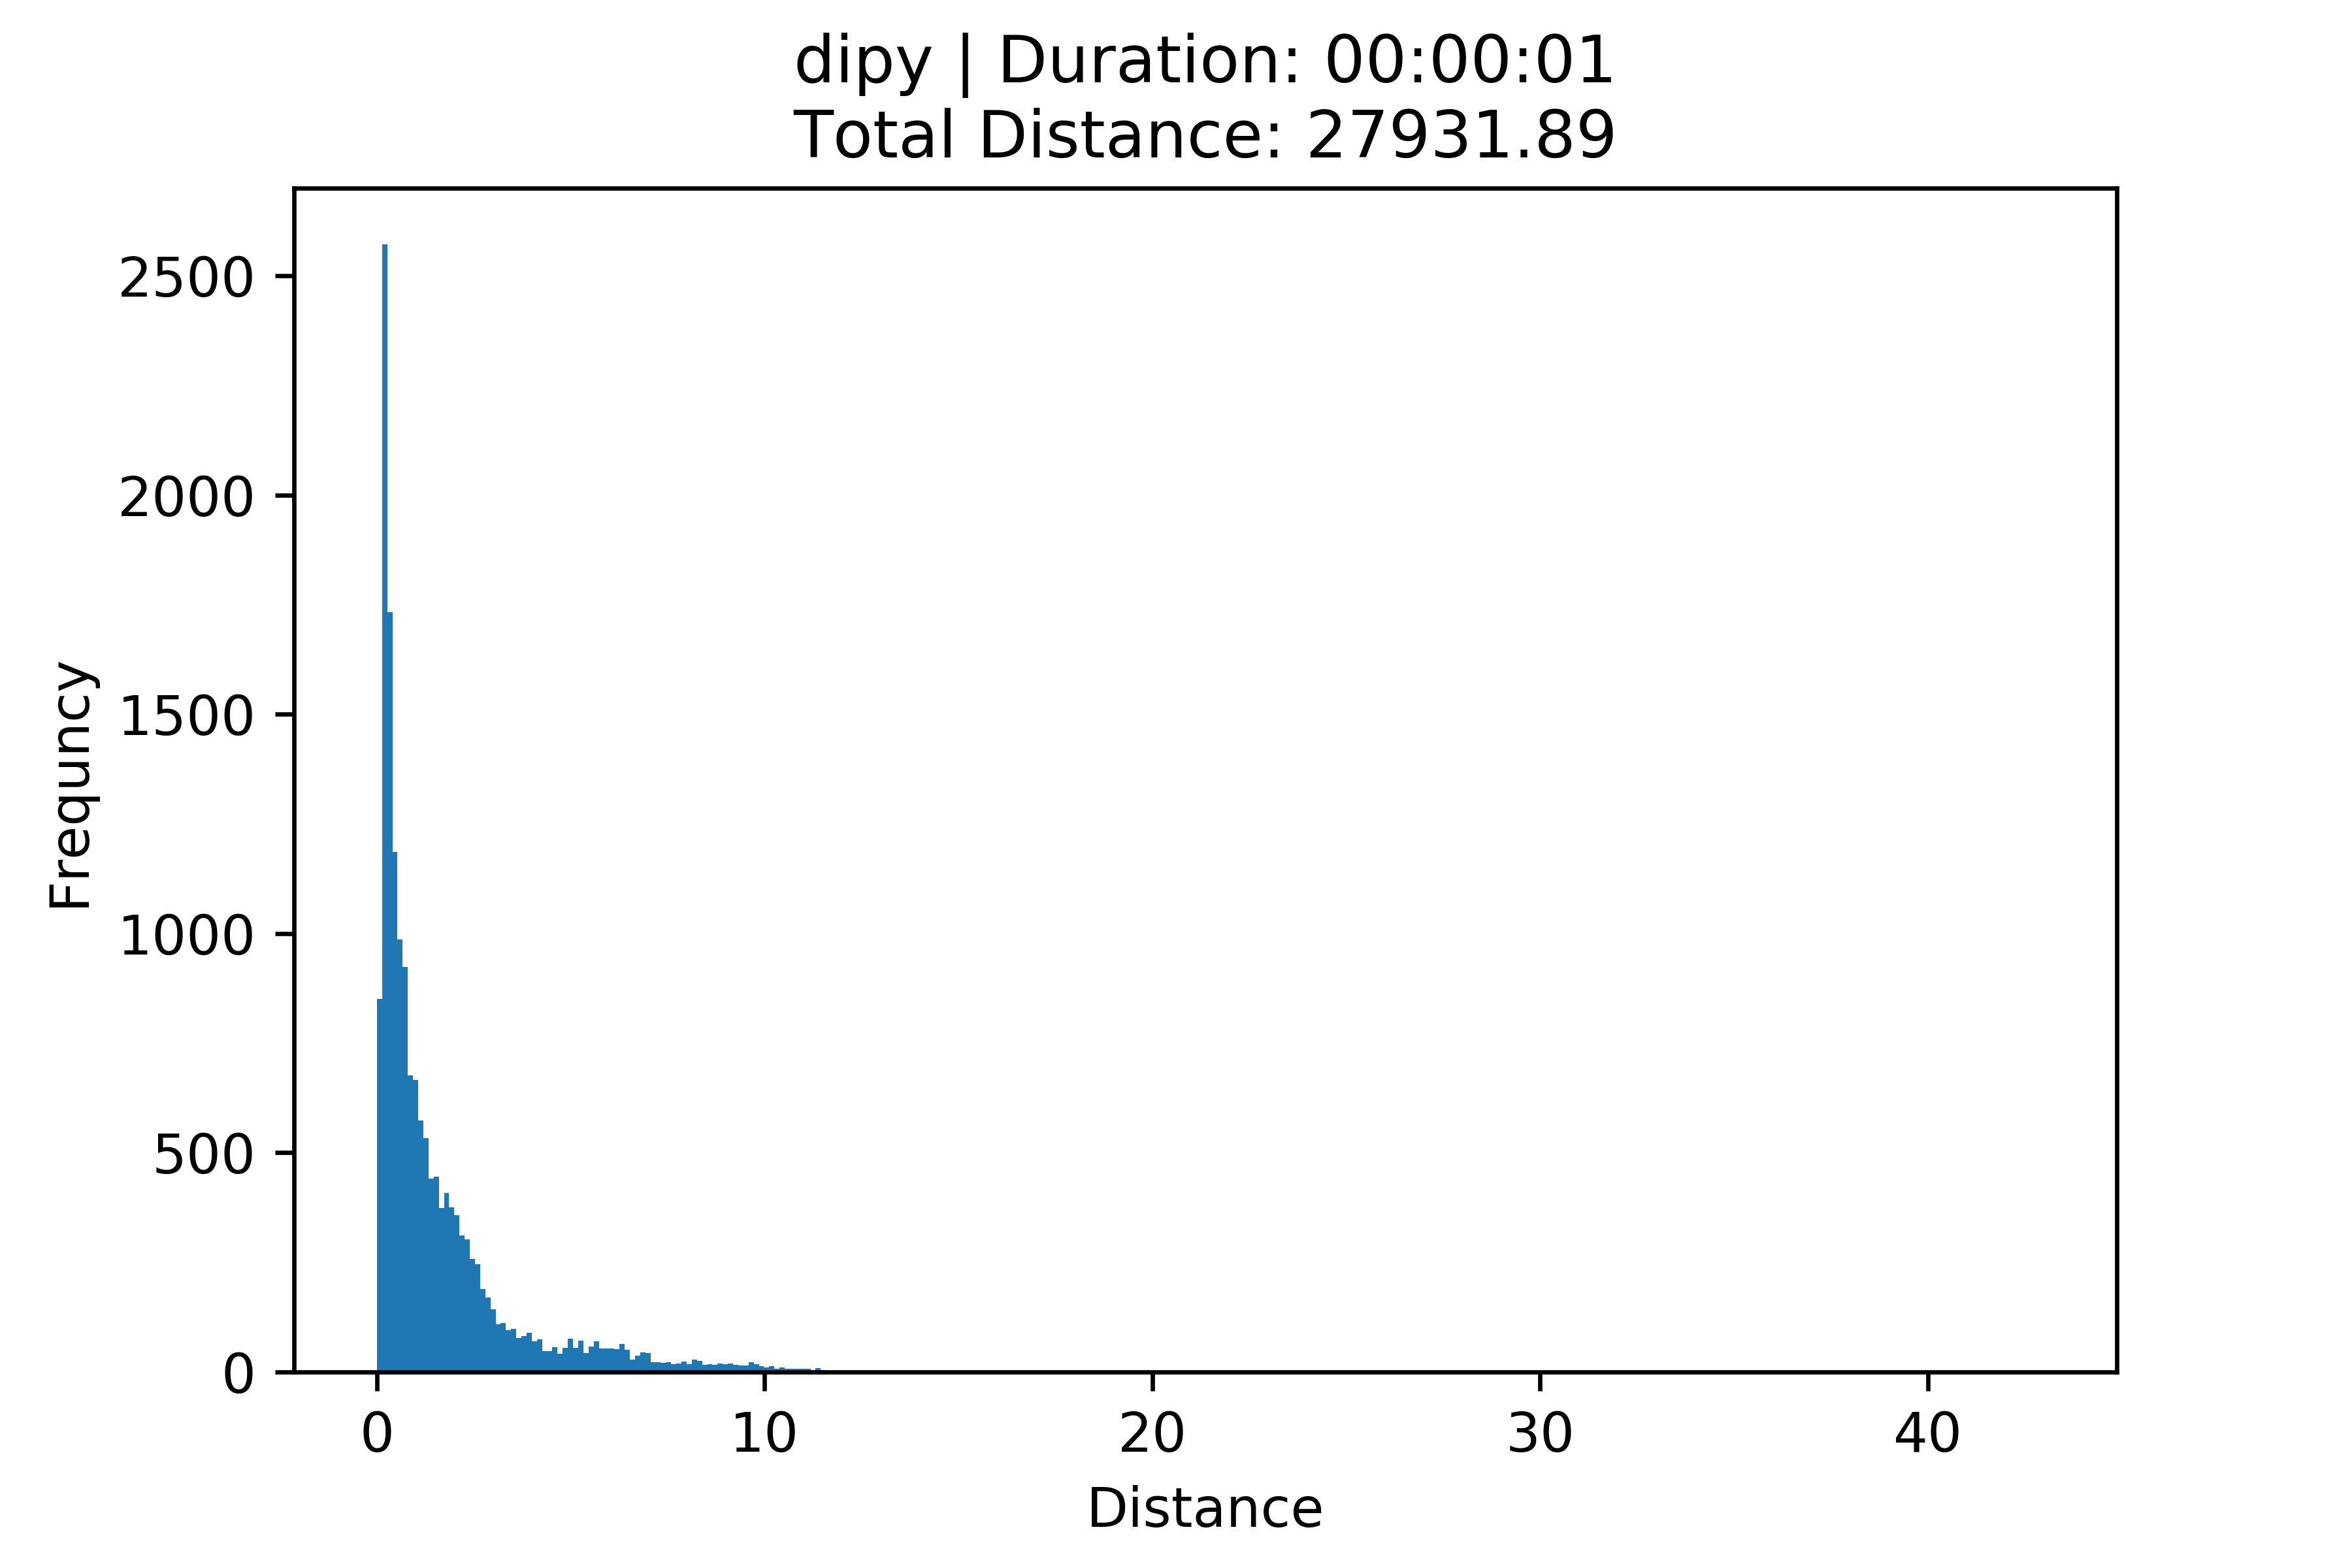
\includegraphics[scale=1]{101_dipy_hist}
\captionsetup{justification=centering}
\caption{The distances histogram after DIPY}
\label{fig:dipy_hist}
\end{figure}

\begin{figure}[h!]
\centering
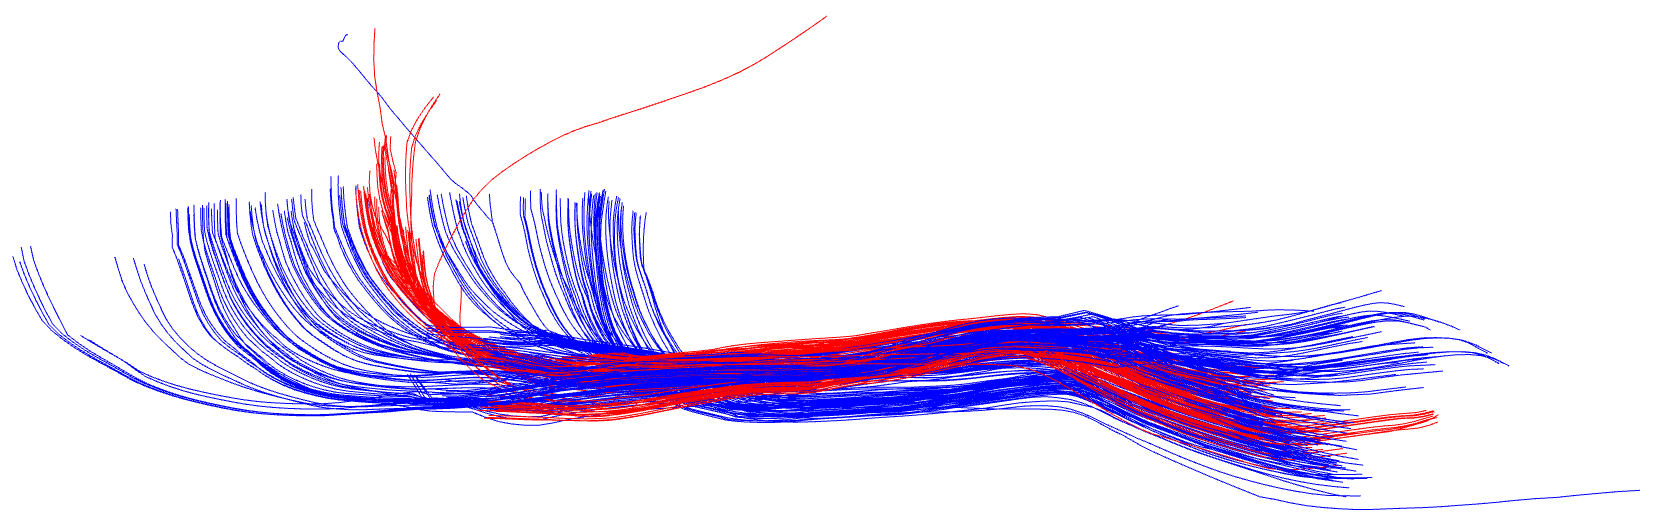
\includegraphics[scale=.3]{101_img_dipy}
\captionsetup{justification=centering}
\caption{The Orientation after DIPY}
\label{fig:img_dipy}
\end{figure}
\pagebreak

The second test is done for the right side of the ATR by transforming it locally and globally. Essentially, what we mean by local transformation is that we apply different affine transformation matrices for each point in the bundle and local means one affine transformation matrix for all points (no deformation). Then we try to align it again with the original one. We show the results in figures \{\ref{fig:hist_original_def}\} \{\ref{fig:img_original_def}\} of local transformation only because it is relatively straightforward for global transformation.

\begin{figure}[h!]
\centering
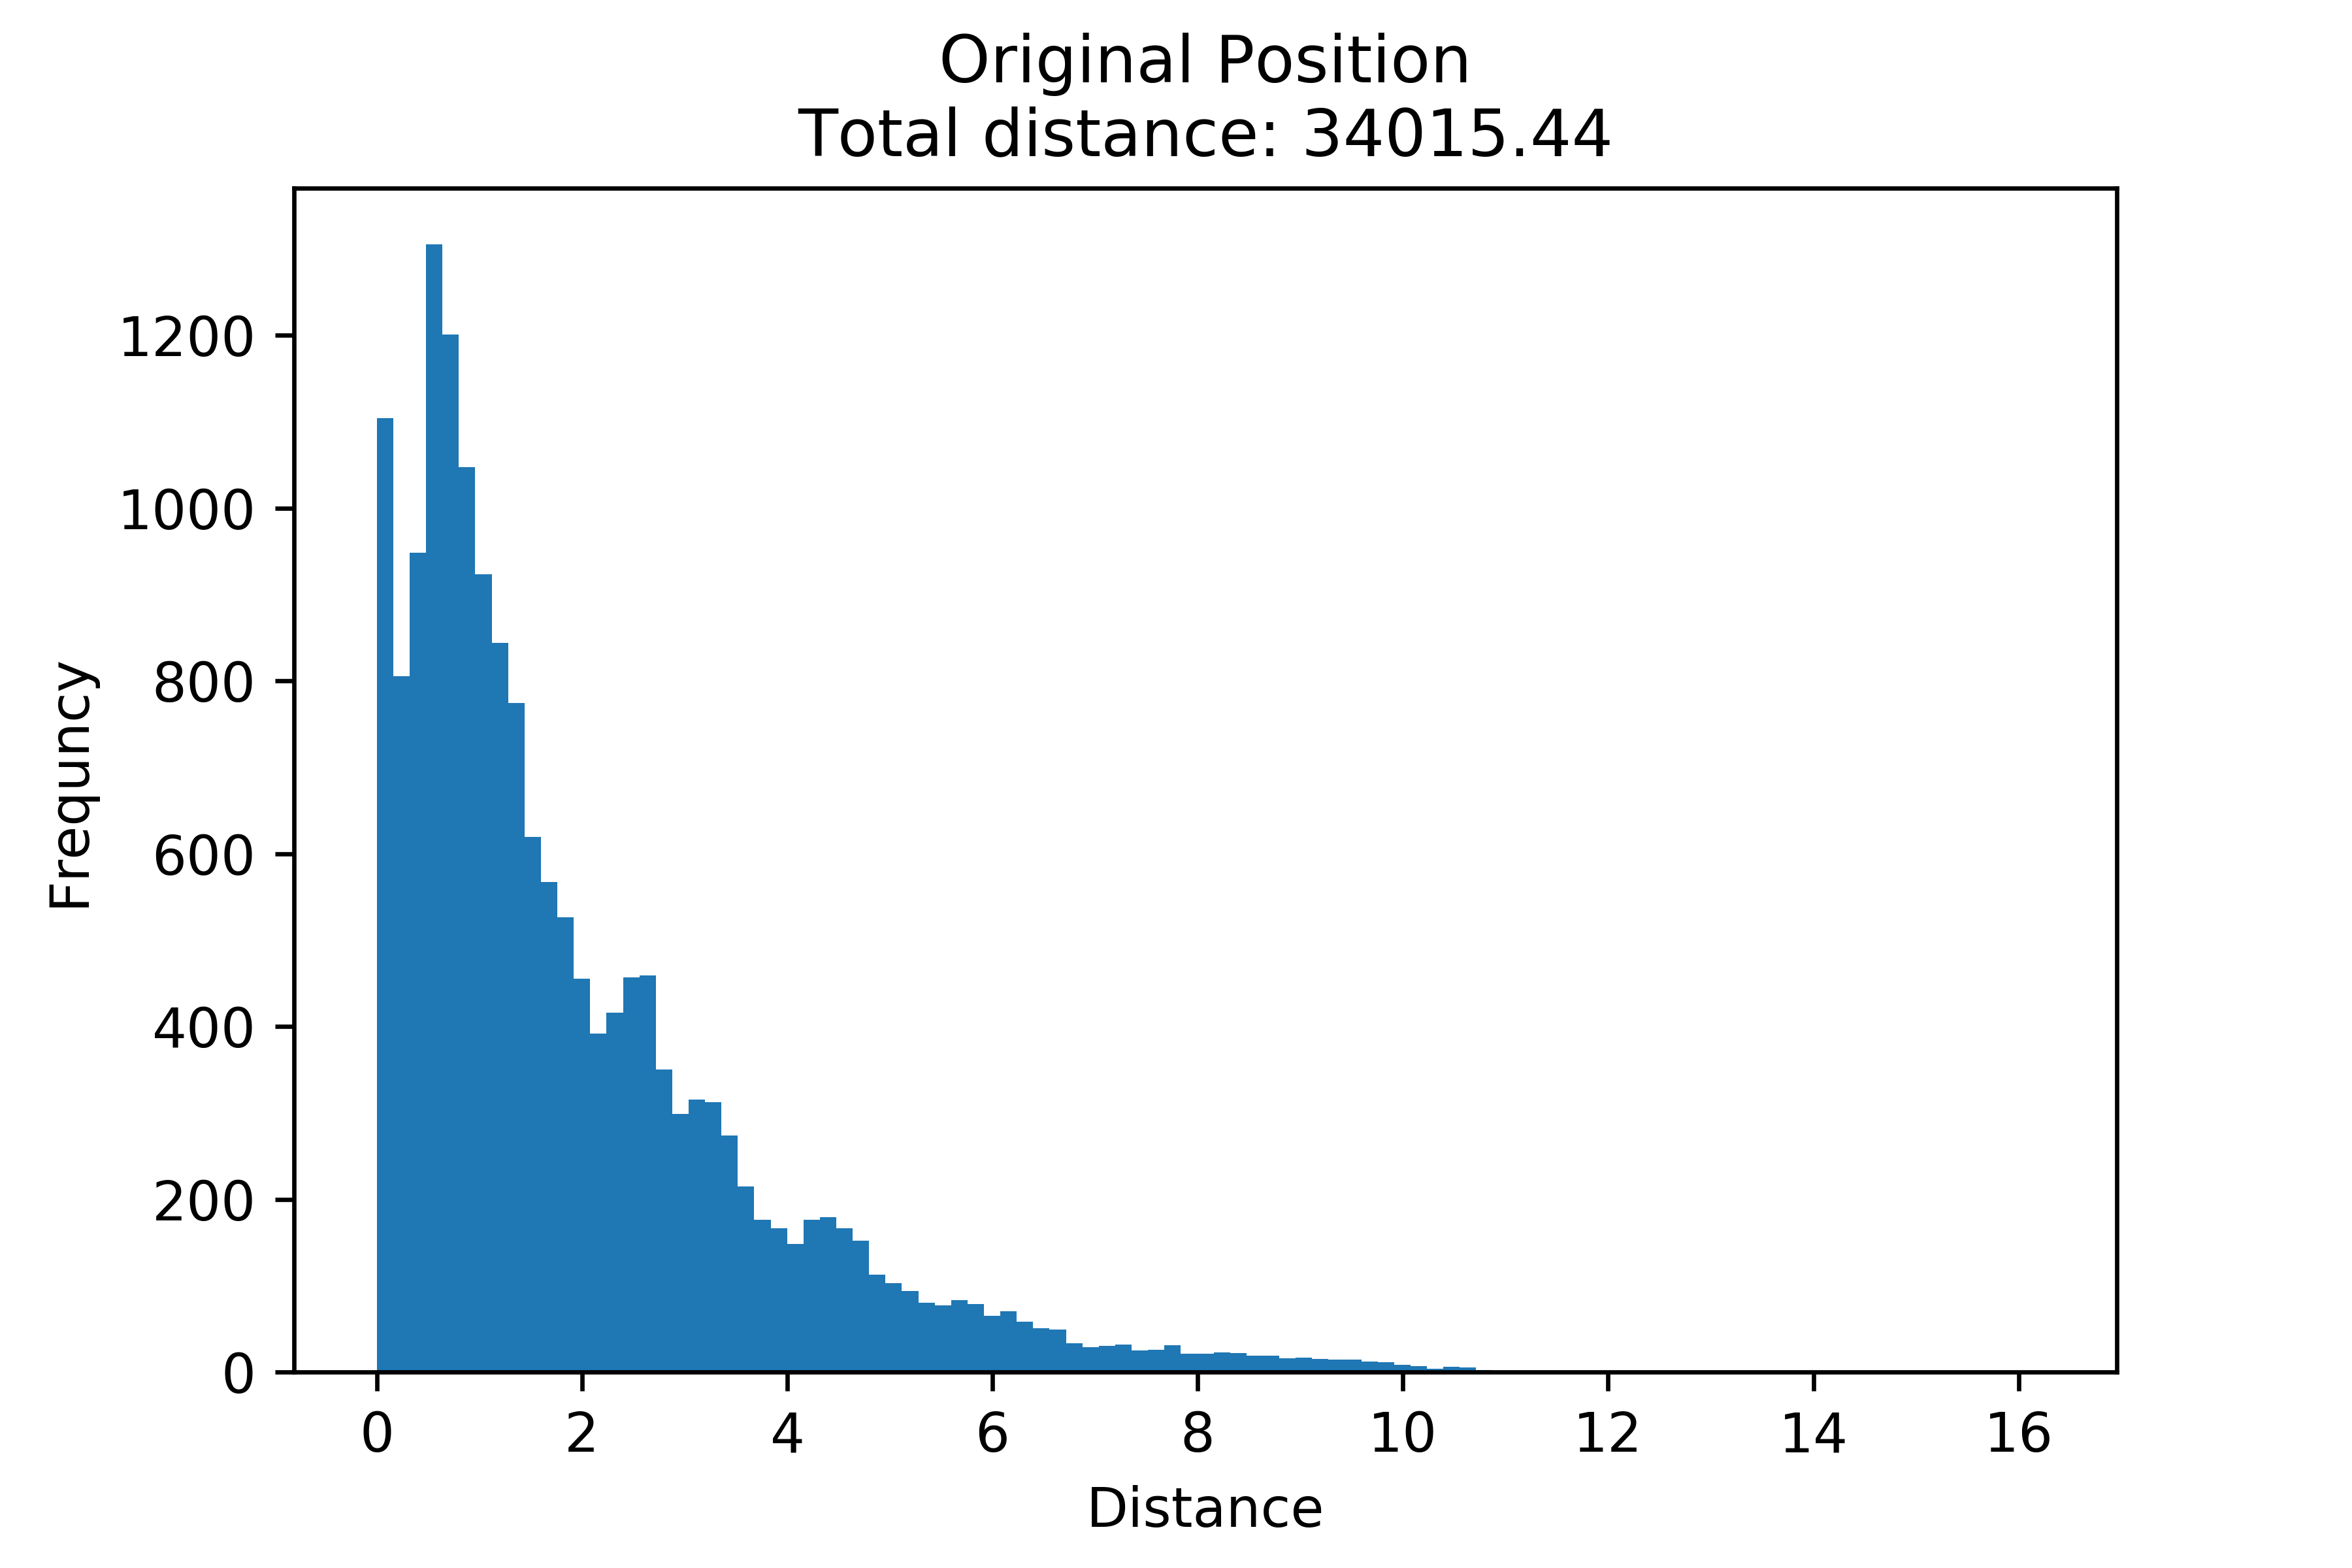
\includegraphics[scale=1]{102_hist_original}
\captionsetup{justification=centering}
\caption{The distances histogram after deforming a bundle and measuring the distances from the original one}
\label{fig:hist_original_def}
\end{figure}

\begin{figure}[h!]
\centering
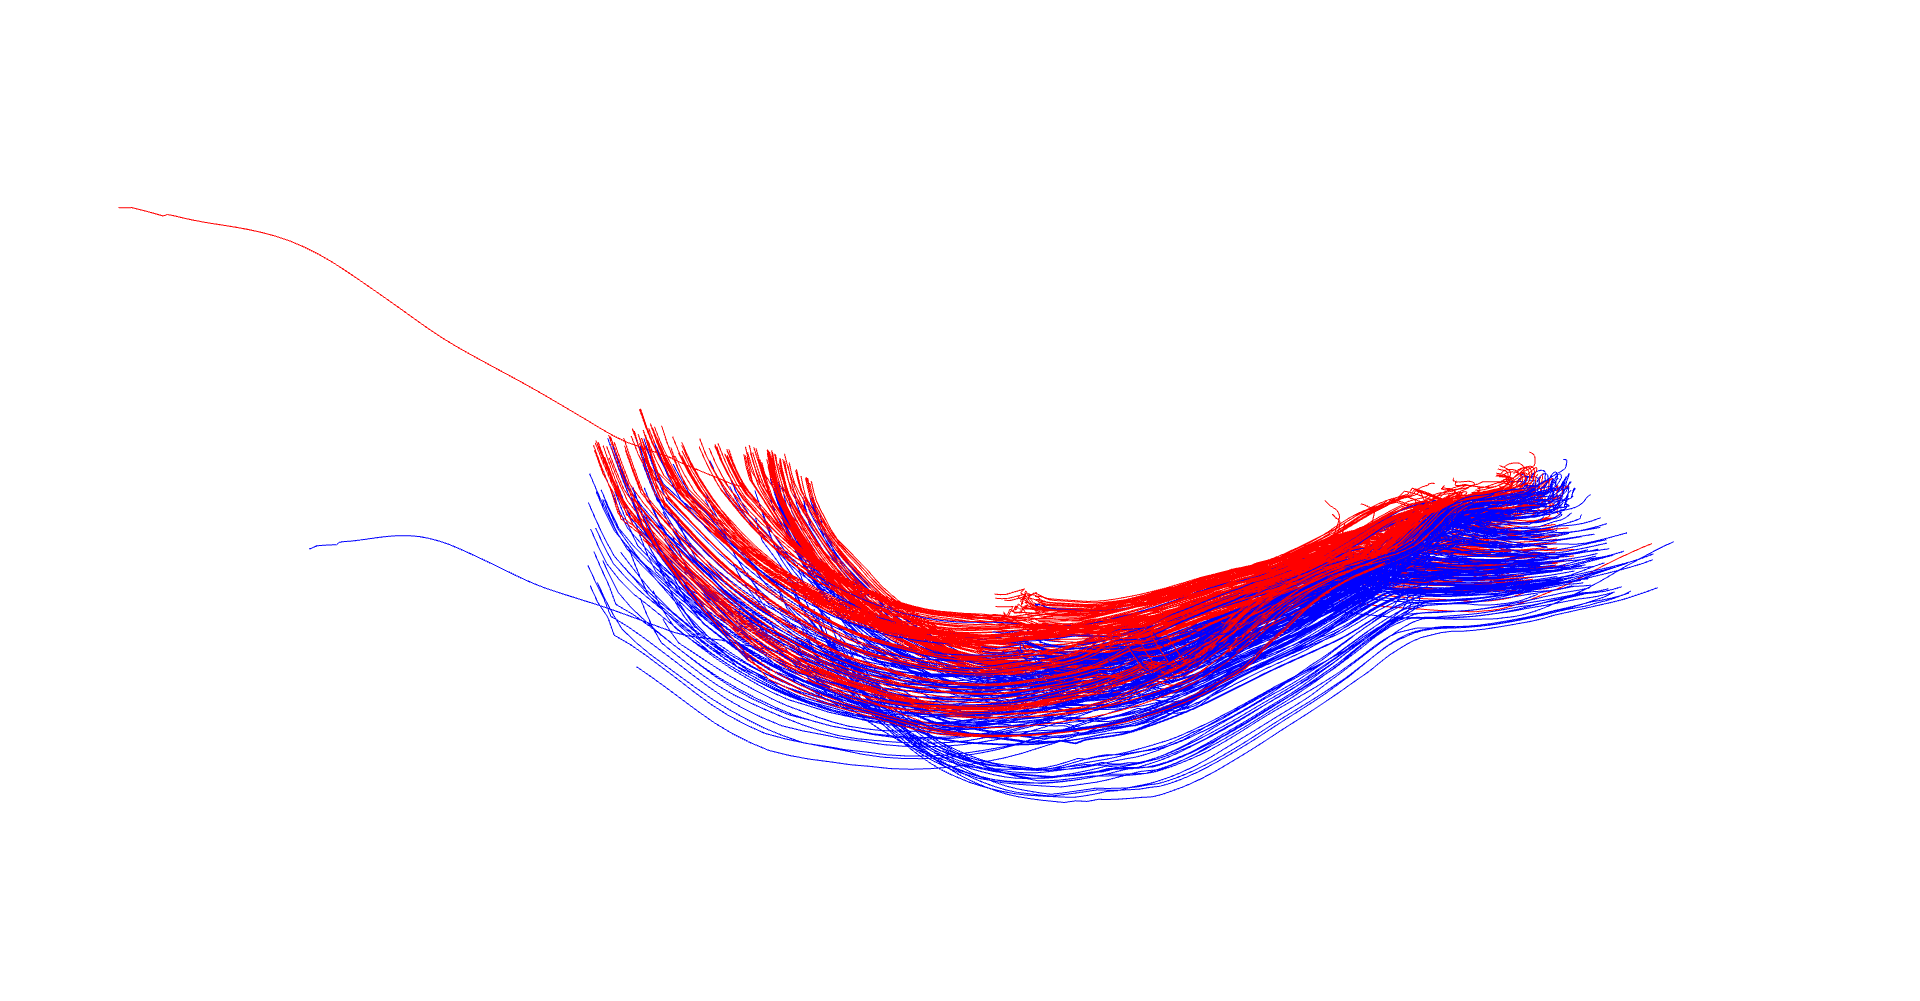
\includegraphics[scale=.3]{102_img_original}
\captionsetup{justification=centering}
\caption{The orientation after deformation}
\label{fig:img_original_def}
\end{figure}
\pagebreak

Next, we align them with DIPY to get the results in figures \{\ref{fig:hist_dipy_def}\} \{\ref{fig:img_dipy_def}\}

\begin{figure}[h!]
\centering
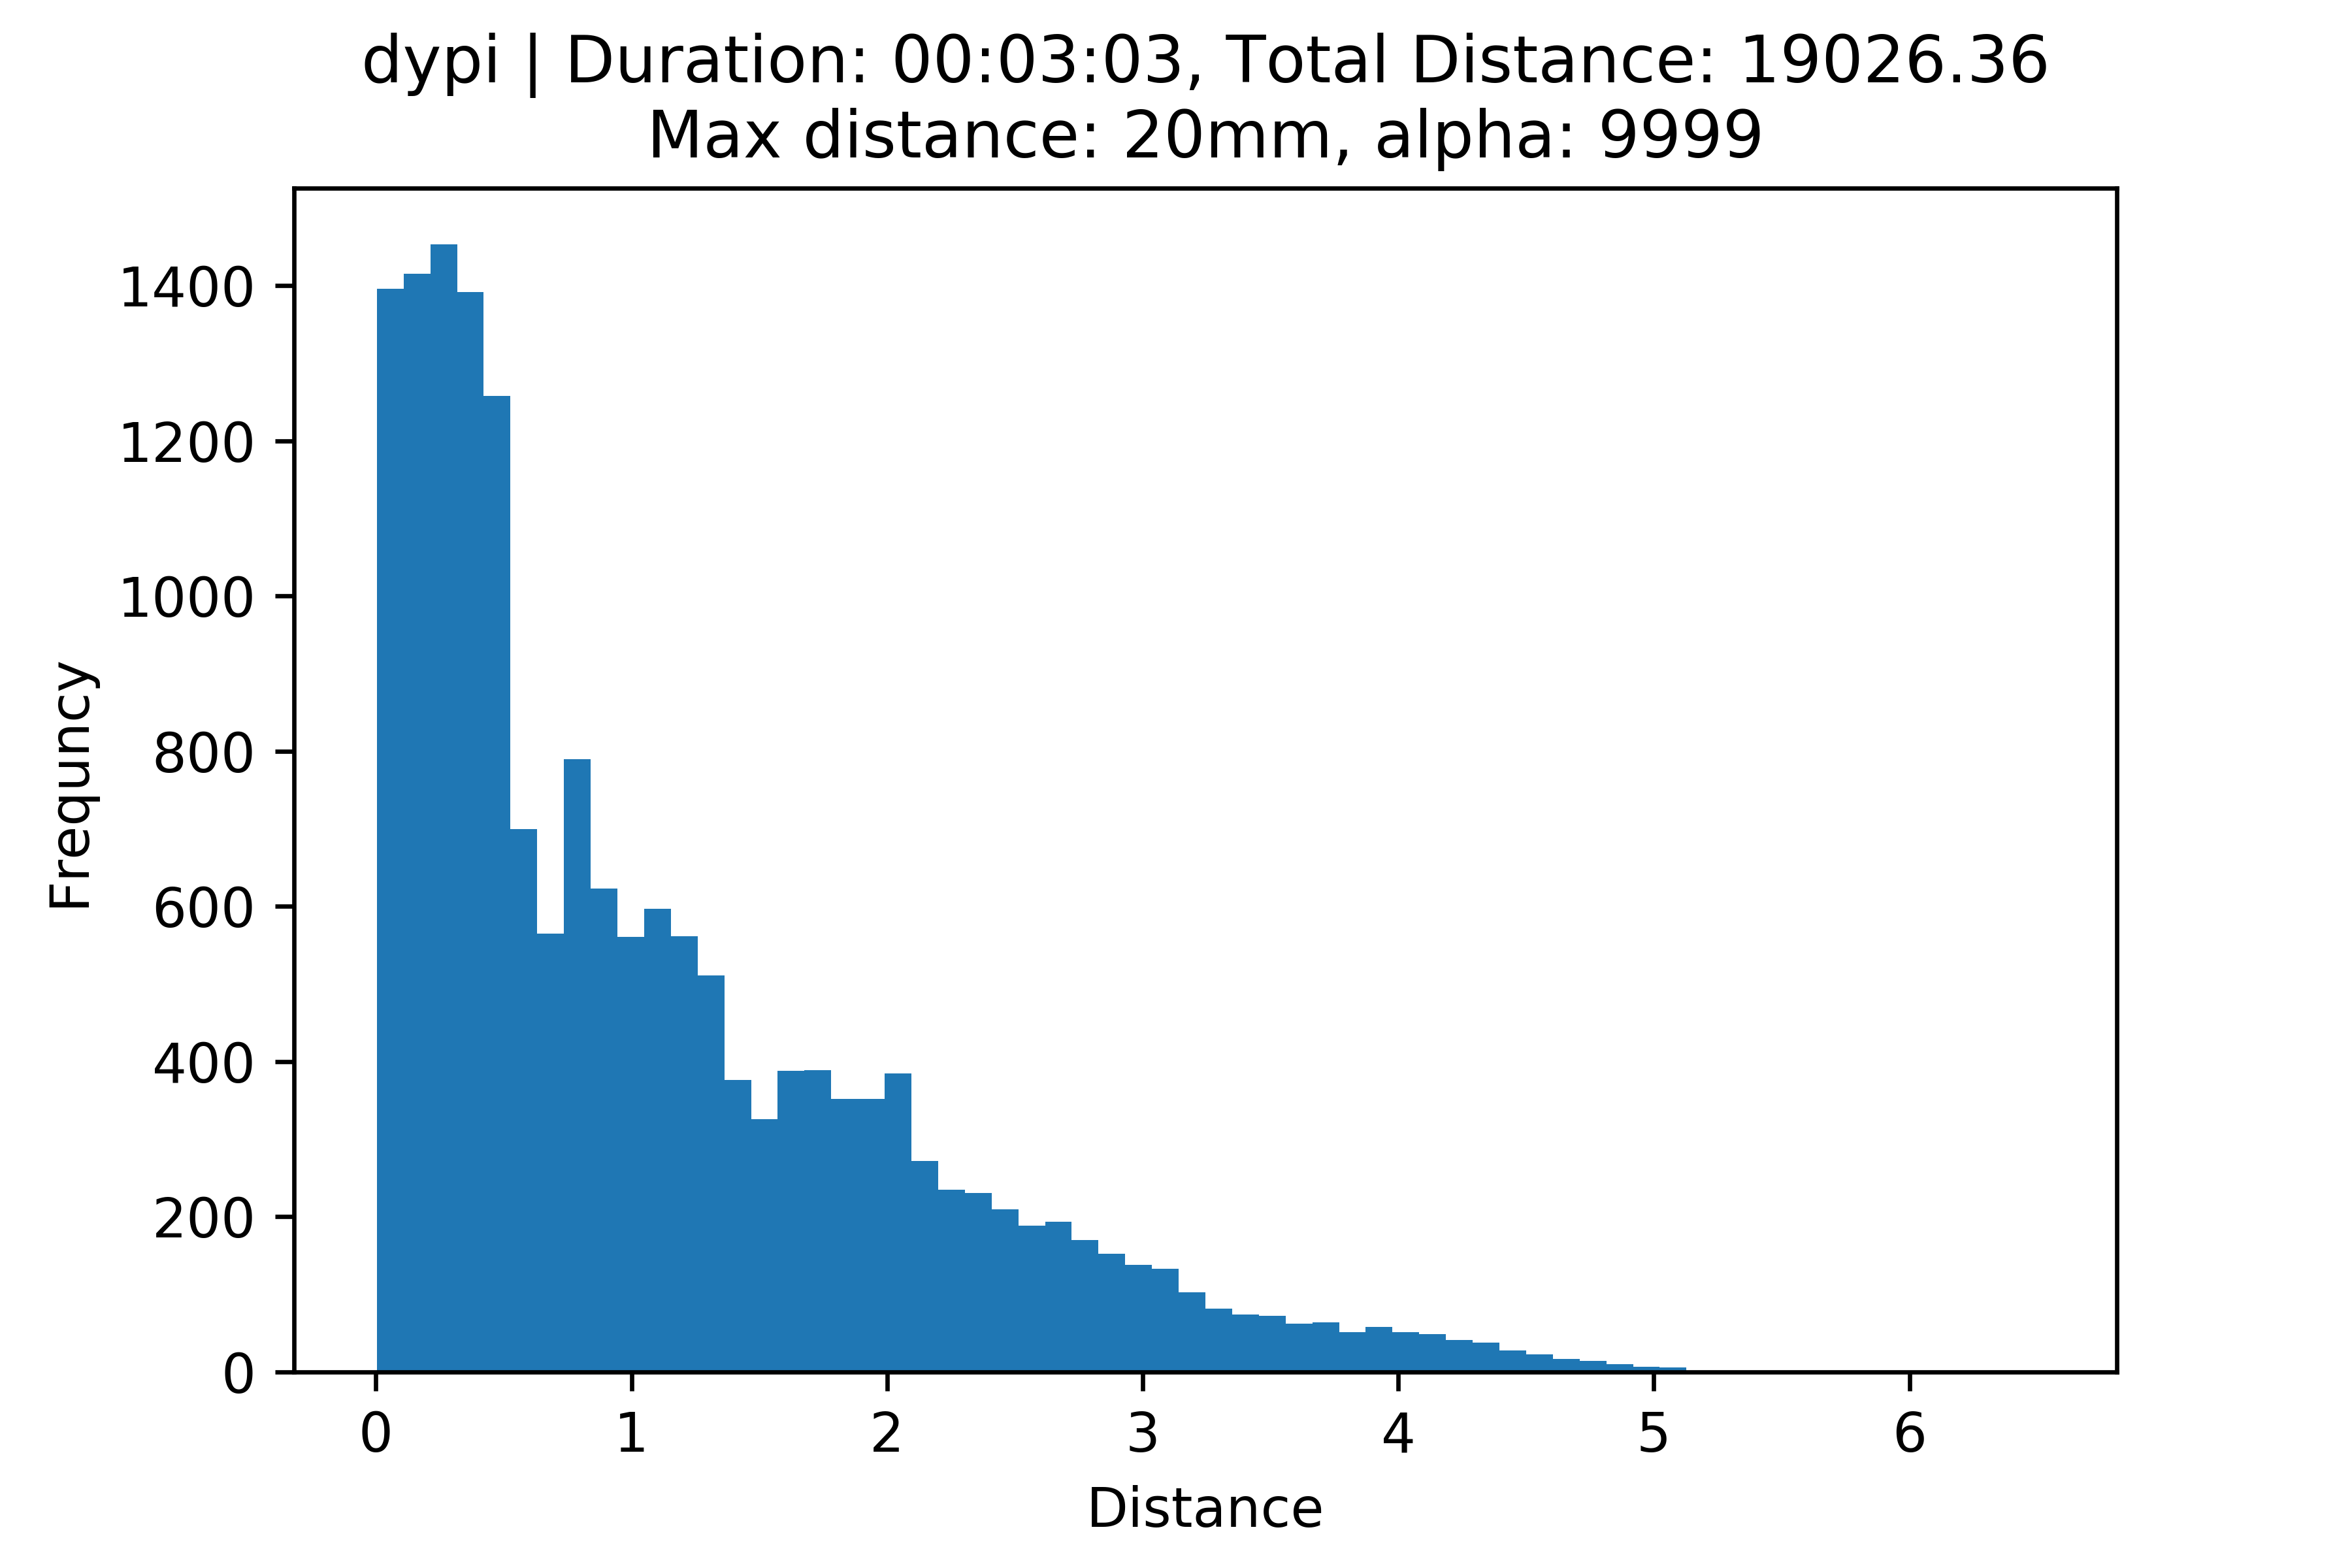
\includegraphics[scale=1]{102_hist_dipy}
\captionsetup{justification=centering}
\caption{The distances histogram after deforming a bundle and aligning it with the original one using DIPY}
\label{fig:hist_dipy_def}
\end{figure}

\begin{figure}[h!]
\centering
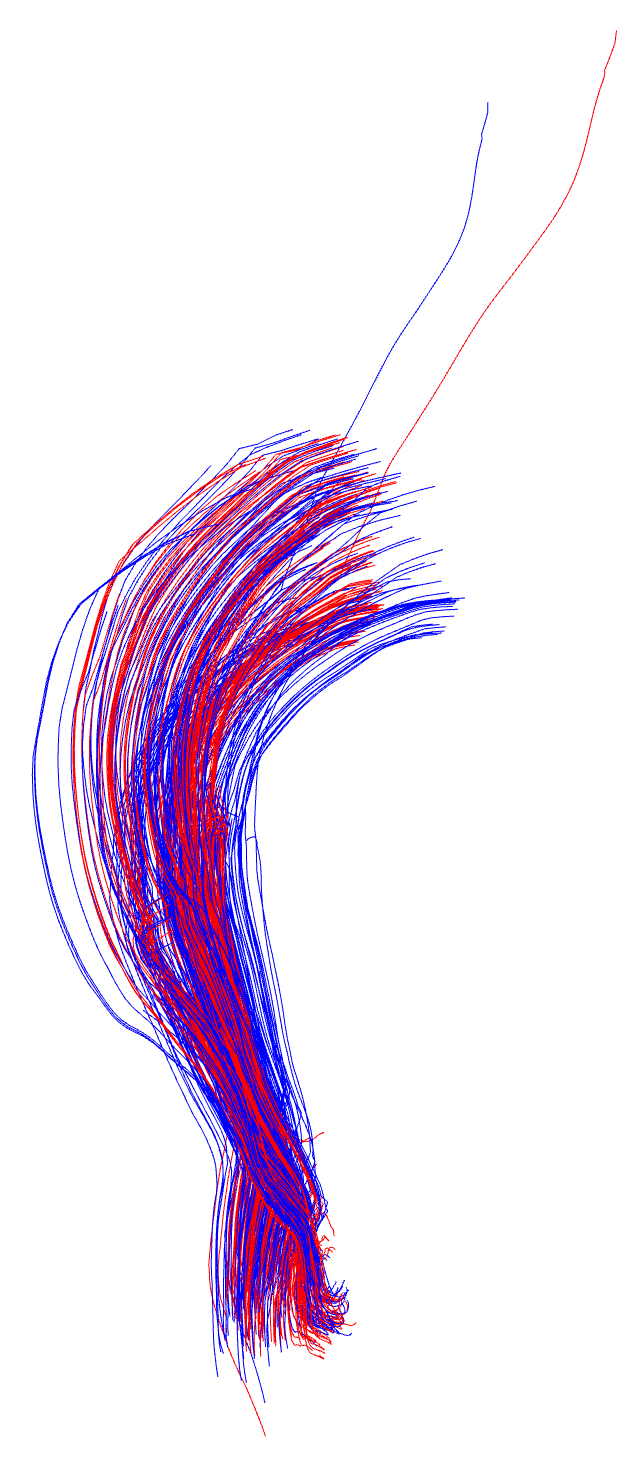
\includegraphics[scale=.3]{102_img_dipy}
\captionsetup{justification=centering}
\caption{The orientation after deforming a bundle and aligning it with the original one using DIPY}
\label{fig:img_dipy_def}
\end{figure}
\pagebreak
We then apply non-rigid ICP registration to get the results in figures \{\ref{fig:hist_icp_def}\} \{\ref{fig:img_icp_def}\}

\begin{figure}[h!]
\centering
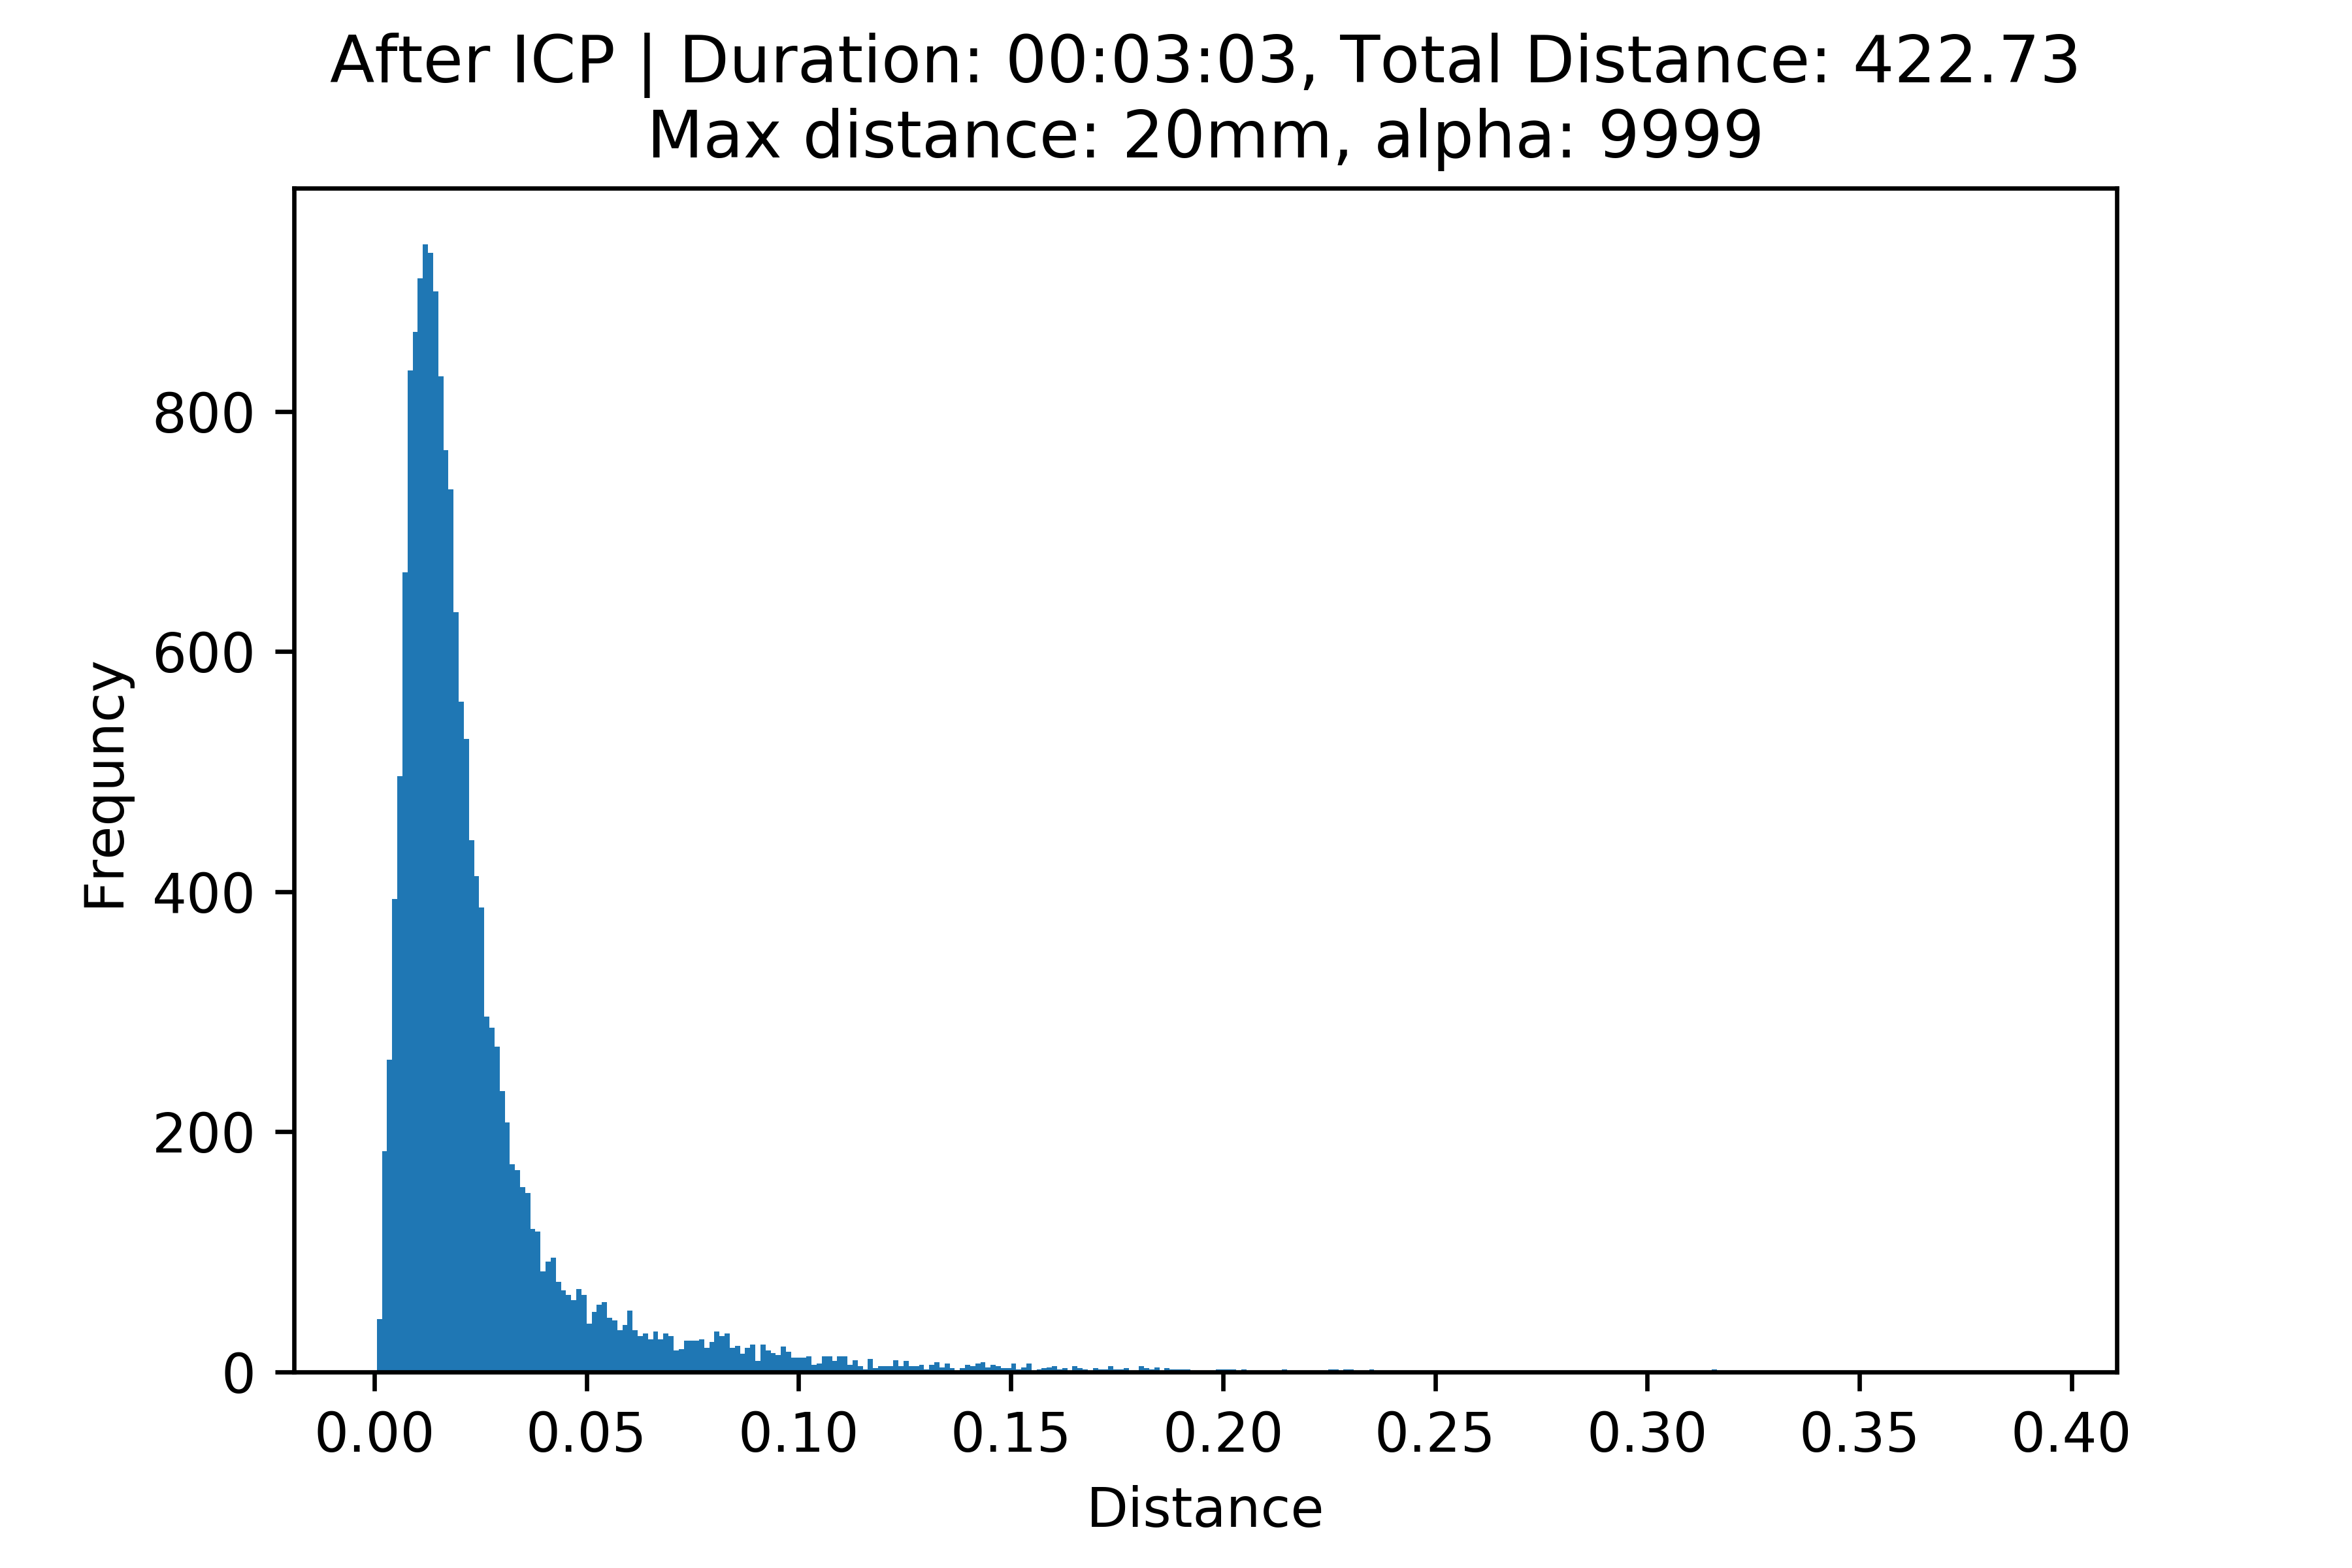
\includegraphics[scale=1]{102_hist_ICP}
\captionsetup{justification=centering}
\caption{The distances histogram after deforming a bundle and aligning it with the original one using ICP}
\label{fig:hist_icp_def}
\end{figure}

\begin{figure}[h!]
\centering
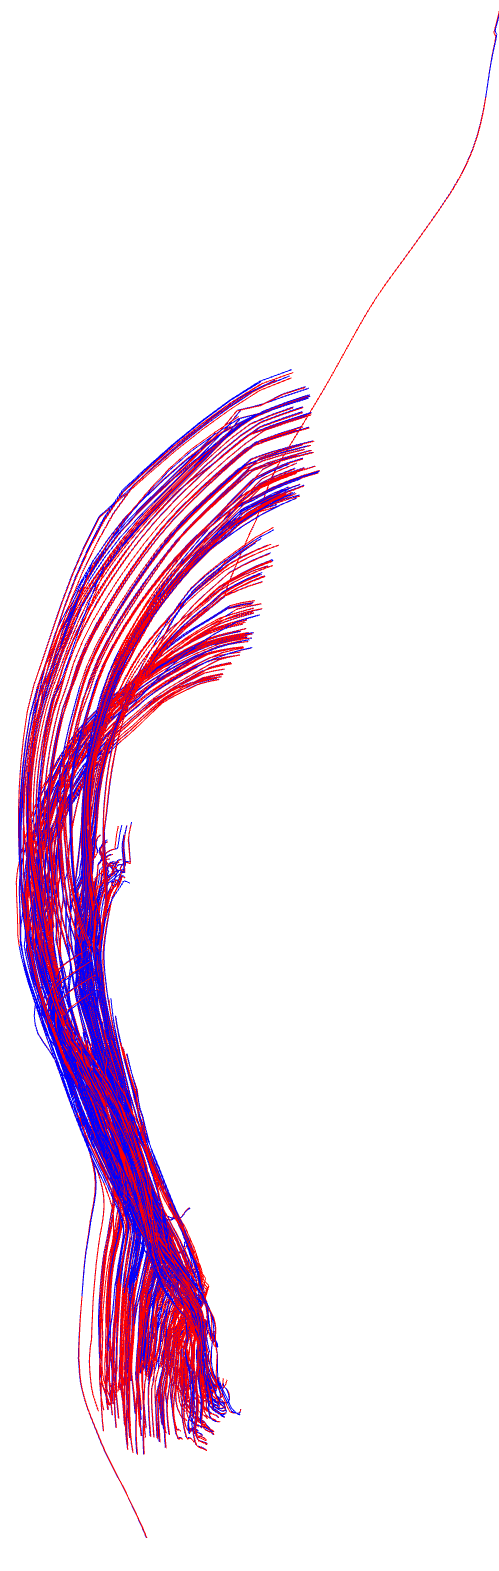
\includegraphics[scale=.3]{102_img_ICP}
\captionsetup{justification=centering}
\caption{The orientation after deforming a bundle and aligning it with the original one using ICP}
\label{fig:img_icp_def}
\end{figure}

\pagebreak

Applying PCA sometimes does not find the right orientation of bundles due to similarity of vertices distribution and that gives similar principle components as shown below:


	\begin{figure}[h!]
	\centering
	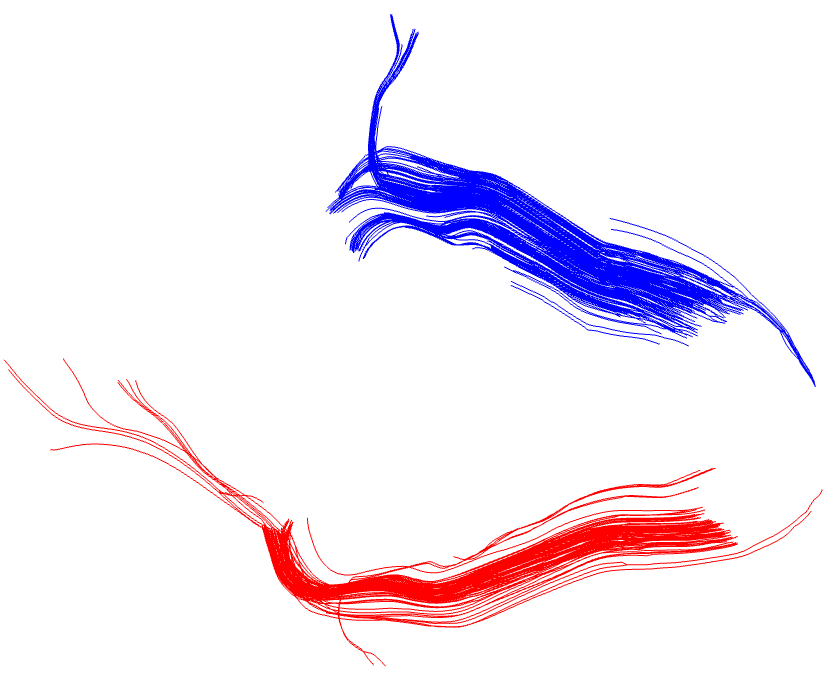
\includegraphics[scale=0.5]{02_img_original}
	\captionsetup{justification=centering}
	\caption{The original coordinate before PCA}
	\label{fig:all_brain}
	\end{figure}
	
	\begin{figure}[h!]
	\centering
	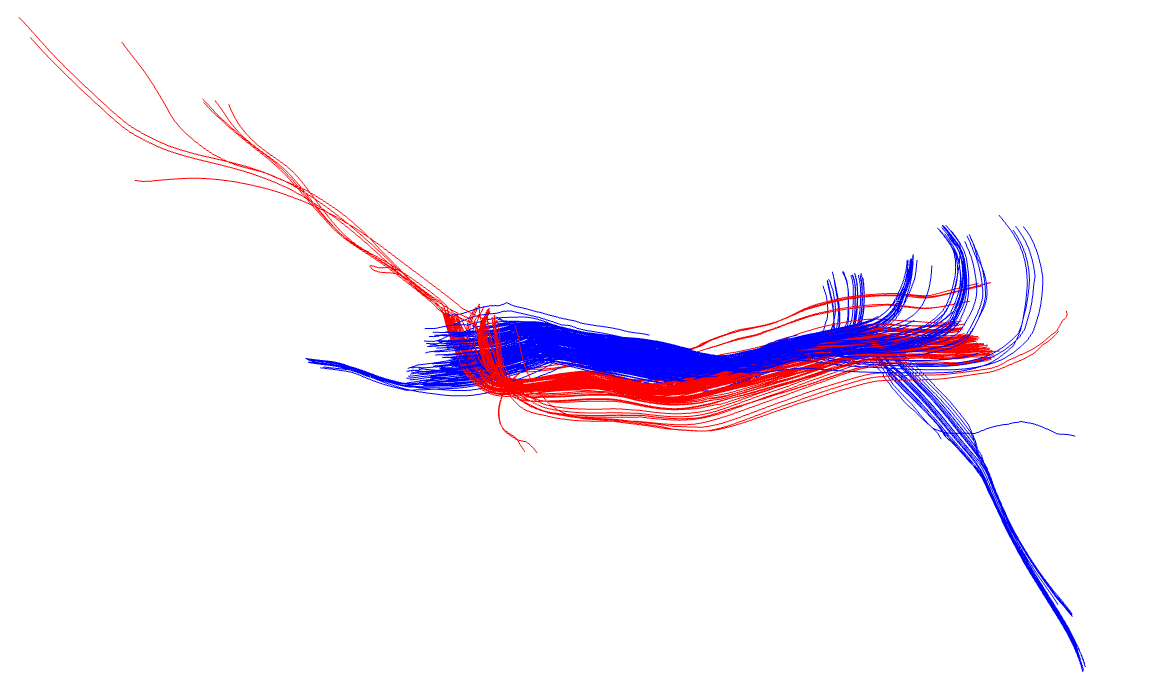
\includegraphics[scale=0.3]{02_img_PCA}
	\captionsetup{justification=centering}
	\caption{The coordinate when PCA fails to find the best alignment}
	\label{fig:all_brain}
	\end{figure}
\pagebreak

Finally, we found that our tool can handle the deformation easily (elastic registration) but \textit{DIPY} can only handle the size by scaling the template bundles.

The \textit{DIPY} method is much faster than our method because it is implemented to reduce the number of points used to calculate the distance. In our test, each tract reduced to 20 points rather than the real number of points as shown in table \{\ref{table:data}\}. Furthermore, as mentioned in \cite{ODonnell2012}, \textit{DIPY} uses a minimum average direct-flip distance (MDF) which considers the tract to tract distance whereas our tool considers the point to point distance. To improve our tool, hierarchical clustering bundles can be done and soft membership alignment can be applied.

\end{document}


